%%%%%%%%%%%%%%%%%%%%%%%%%%%%%%%%%%%%%%%%%%%%%%%%%%%% 1.o Esempio con la classe toptesi
\documentclass[12pt,twoside,cucitura]{toptesi}
%\documentclass[twoside,cucitura,pdfa]{toptesi}
%%%%%%%%%%%%%%%%%%%%%%%%%%%%%%%%%%%%%%%%%%%%%%%%%%%% 2.o Esempio con la classe toptesi
% \documentclass[11pt,twoside,oldstyle,autoretitolo,classica,greek]{toptesi}
% \usepackage[or]{teubner}
%%%%%%%%%%%%%%%%%%%%%%%%%%%%%%%%%%%%%%%%%%%%%%%%%%%%
% Commentare la riga seguente se si � specificata l'opzione "pdfa"
\usepackage{hyperref}
\hypersetup{%
    pdfpagemode={UseOutlines},
    bookmarksopen,
    pdfstartview={FitH},
    colorlinks,
    linkcolor={blue},
    citecolor={red},
    urlcolor={blue}
  }

\usepackage{toptesi}

%\usepackage{times}
\usepackage{algorithm}
\usepackage{algorithmic}
%\usepackage{algorithmicx}

\usepackage{acronym}
\usepackage{xspace}

\usepackage{graphicx}
\usepackage{epstopdf}
\usepackage{multirow}
\usepackage{amssymb, amsmath}
%\usepackage{enumerate}
\usepackage{url}
%\usepackage{natbib}
%\usepackage{ecrc}
\usepackage{subfigure}
\usepackage{dblfloatfix}
\usepackage{epsfig}
\usepackage{color}
\usepackage{fancyvrb}
\DefineVerbatimEnvironment{code}{Verbatim}{fontsize=\tiny}

%\usepackage{algpseudocode}

\usepackage{paralist}
\usepackage{ctable}
\usepackage{rotating}
\usepackage{cite}
\usepackage{appendix}
\usepackage[latin1]{inputenc}
\usepackage[english]{babel}
\input{kvmacros}


\usepackage{framedbox}
\usepackage{subfigure}
\usepackage{slashbox}
\usepackage{pifont}
\usepackage[multiple]{footmisc}

\usepackage[T1]{fontenc}
\usepackage{times}%
\usepackage{topcapt}
\usepackage{natbib}% for bibliography sorting/compressing
%\usepackage{pdfpages}
%\usepackage{amsmath}
%\usepackage{endnotes}
\usepackage{graphics}


%\usepackage{times}
\newcounter{eqn}
\renewcommand*{\theeqn}{\alph{eqn})}
\newcommand{\num}{\refstepcounter{eqn}\text{\theeqn}\;}

\makeatletter
%\newcommand{\putindeepbox}[2][0.7\baselineskip]{{%
\newcommand{\putindeepbox}[2][scale=0.4]{{%
    \setbox0=\hbox{#2}%
    \setbox0=\vbox{\noindent\hsize=\wd0\unhbox0}
    \@tempdima=\dp0
    \advance\@tempdima by \ht0
    \advance\@tempdima by -#1\relax
    \dp0=\@tempdima
    \ht0=#1\relax
    \box0
}}
\makeatother




\usepackage{multirow}
\usepackage{amssymb, amsmath}
%\usepackage{enumerate}
%\usepackage{url}
%\usepackage{color} 
\usepackage{listings}
%\usepackage{paralist}
%\usepackage{ctable}



% Scritto in italiano con la classe inglese
%\inglese
%\setcaptions
  
%
% Esempio di composizione di tesi di laurea con PDFLATEX <---------------- !
%
% Questo esempio e' stato preparato inizialmente 13-marzo-1989
% e poi e' stato modificato via via che TOPtesi andava
% arricchendosi di altre possibilita'.
%
% Per comporre con XeLaTeX, invece che con pdfLaTeX, vedere il file toptesi-example-xetex.tex
% A parte i font, bisogna specificare alcune cose dopo la fine del preambolo.
%
% Nel seguito laurea "quinquennale" sta anche per "specialistica" o "magistrale".
%
% Cambiare encoding a piacere; oppure non caricare nessun encoding se si usano
% solo caratteri a 7 bit (ASCII) nei file d'entrata.
%
%\usepackage[ansinew]{inputenc}% per macchine Windows
\usepackage{lmodern}



	\ateneo{POLITECNICO DI TORINO}
	\facolta{Elettronica e Telecomunicazioni}
 	\titolo{Design and Implementation of OFDM System on FPGA}
 	\sottotitolo {}
 	\corsodilaurea{Electronic and Telecommunication Engineering}
 	
 	\candidato{Seyed-Ehsan Koohestani}
 	\coordinatore{Prof. M. Mondin, Prof. R. Garello, Prof. A. K. Khandani}
 	\tutore{Prof. Marina Mondin - Prof. Roberto Garello - Prof. Amir Keyvan Khandani}
 	 	
 	\esamedidottorato{March 2015}
 	%\ciclodidottorato{XXVI Ciclo}
 	
 	\logosede{logopolito.eps}
 	
%
%%\ateneo{Universit{\`a} degli Studi di Trieste}
%\facolta[III]{Matematica, Fisica\\e Scienze Naturali}
%%\Materia{Remote sensing}
%%\monografia{La pressione barometrica di Giove}% per la laurea triennale
%\titolo{La pressione barometrica di Giove}% per la laurea quinquennale e il dottorato
%\sottotitolo{Metodo dei satelliti medicei}% per la laurea quinquennale e il dottorato
%\corsodilaurea{Astronomia Applicata}% per la laurea
%%\corsodidottorato{Meccanica}% per il dottorato
%\candidato{Galileo \textsc{Galilei}}% per tutti i percorsi
%\secondocandidato{Evangelista \textsc{Torricelli}}% per la laurea magistrale solamente
%%\direttore{prof. Albert Einstein}% per il dottorato
%%\coordinatore{prof. Albert Einstein}% per il dottorato
%\relatore{prof.\ Albert Einstein}% per la laurea e/o il dottorato
%\secondorelatore{dipl.~ing.~Werner von Braun}% per la laurea magistrale
%%\terzorelatore{{\tabular{@{}l}dott.\ Neil Armstrong\\prof. Maria Rossi\endtabular}}% per la laurea magistrale
%%\tutore{ing.~Karl Von Braun}% per il dottorato
%\tutoreaziendale{dott.\ ing.\ Giovanni Giacosa}
%\NomeTutoreAziendale{Supervisore aziendale\\Centro Ricerche FIAT}
%%\sedutadilaurea{Agosto 1615}% per la laurea quinquennale
%%\esamedidottorato{Novembre 1610}% per il dottorato
%\sedutadilaurea{\textsc{Anno~accademico} 1615-1616}% per la laurea magistrale
%%\annoaccademico{1615-1616}% solo con l'opzione classica
%%\annoaccademico{2006-2007}% idem
%\ciclodidottorato{XV}% per il dottorato
%\logosede{logopolito}% questo e' ovviamente facoltativo, ma e' richiesto per il dottorato al PoliTO
%%
%%\chapterbib %solo per vedere che cosa succede; e' preferibile comporre una sola bibliografia
%%\AdvisorName{Supervisors}
\newtheorem{osservazione}{Osservazione}% Standard LaTeX
 	


\newcommand{\figref}[1] {Fig.~\ref{#1}}
\newcommand{\secref}[1] {Section~\ref{#1}}
\newcommand{\tabref}[1] {Table~\ref{#1}}
\newcommand{\eqtnref}[1] {Eq.~\ref{#1}}
\newcommand{\algref}[1] {Alg.~\ref{#1}}

\newcommand{\refnet}{base network\xspace}
\newcommand{\germany}{Germany17\xspace}
\newcommand{\abilene}{Abilene\xspace}
\newcommand{\geant}{G\'{e}ant\xspace}

\newcommand{\myparagraph}[1]{\par{\textbf{#1}}}

\newcommand{\nobel} {{\sc Nobel}\xspace}
\newcommand{\zimpl} {{\sc Zimpl}\xspace}
\newcommand{\cplex} {{\sc Cplex}\xspace}
%% ----------------------------------------------------------------------
%%    general math
%% ----------------------------------------------------------------------
\renewcommand{\implies}{\ensuremath{\Rightarrow}}
\newcommand{\R}            {\ensuremath{\mathbb{R}}\xspace}
\newcommand{\Rplus}        {\ensuremath{\R_+}\xspace}
\newcommand{\Z}            {\ensuremath{\mathbb{Z}}\xspace}
\newcommand{\Zplus}        {\ensuremath{\Z_+}\xspace}
\newcommand{\card}[1]      {\ensuremath{\left|{#1}\right|}\xspace}
\newcommand{\abs}[1]       {\ensuremath{\card{#1}}\xspace}
% \newcommand{\norm}[1]      {\ensuremath{\left\|{#1}\right\|}\xspace}
\newcommand{\NP}{NP\xspace}
\newcommand{\NPhard}{\NP -hard\xspace}

\renewcommand {\atop} [2] {\genfrac{}{}{0pt}{}{#1}{#2}}

% sets
\newcommand{\set}[1] {\left\{ {#1} \right\}}
%\newcommand{\settype}      [1] {\ensuremath{\mathcal{#1}}\xspace}
\newcommand{\settype}      [1] {\ensuremath{#1}\xspace}
\newcommand{\elementtype}  [1] {\ensuremath{#1}\xspace}

% nodes and edges
\newcommand{\node}             {\elementtype{i}}
\newcommand{\othernode}        {\elementtype{j}}
\newcommand{\physgraph}        {\settype{G}}
\newcommand{\virtgraph}        {\settype{H}}
\newcommand{\nodes}            {\settype{V}}
\newcommand{\allnodepairs}     {\settype{\nodes\times\nodes}}
\newcommand{\physlink}         {\elementtype{e}}
\newcommand{\allphyslinks}     {\settype{E}}
\newcommand{\virtlink}         {\elementtype{l}}
%\newcommand{\allvirtlinks}     {\settype{L}}
\newcommand{\link}          {\elementtype{p}}
\newcommand{\alllinks}          {\elementtype{P}}
\newcommand{\alllinksnodepair}          {\elementtype{\alllinks_{\nodepair}}}
\newcommand{\alllinksending}[1]          {\alllinks_#1}
\newcommand{\allphyslinksending}[1]          {\delta_{\allphyslinks}(#1)}
\newcommand{\alllinksusing}[1]          {\link\in\alllinks:\,#1\in\link}
\newcommand{\alllinkstraversing}[1]          {\alllinks_#1}
\newcommand{\nodepair}          {\elementtype{(\node,\othernode)}}
\newcommand{\linkfwd}          {\elementtype{ij}}
\newcommand{\linkbwd}          {\elementtype{ji}}

\newcommand{\linkweight}          {\elementtype{w_{\virtlink}}}
\newcommand{\demandsrcnode}             {\elementtype{a}}
\newcommand{\demandtrgtnode}             {\elementtype{b}}
\newcommand{\demandsrctrgtnodepair}          {\elementtype{(\demandsrcnode,\demandtrgtnode)}}
\newcommand{\physlinklength}          {\elementtype{L_{\physlink}}}
\newcommand{\physlinkamplifiers}          {\elementtype{N_{a}^{\physlink}}}

% time periods
\newcommand{\period}       {\ensuremath{t}\xspace}
\newcommand{\allPeriods}   {\ensuremath{T}\xspace}
\newcommand{\tinT}         {\ensuremath{\period \in \allPeriods}\xspace}

% demands and commodities
\newcommand{\com}                   {\elementtype{k}}
\newcommand{\allcoms}               {\settype{K}}

% demand values
\newcommand{\demandvalueof} [1]{\ensuremath{d_{#1}}\xspace}
\newcommand{\demandvalueofat} [2]{\ensuremath{d_{#1}}\xspace}
\newcommand{\dij}            {\ensuremath{d_{\node\othernode}}\xspace}
\newcommand{\dki}         {\ensuremath{d_{\com\node}}\xspace}
\newcommand{\demandvalue}    {\settype{\demandvalueof{\demand}}}
\newcommand{\comdemandvalue}   {\ensuremath{\demandvalueof{}^{\com}}\xspace}
\newcommand{\nodedemandvalue}  {\ensuremath{\demandvalueof{\node}^{\com}}\xspace}
\newcommand{\nodeemanatingdemandvalue}  {\ensuremath{\demandvalueof{\node}}\xspace}

\newcommand{\dji}            {\ensuremath{d_{\othernode\node}}\xspace}
\newcommand{\dab}            {\ensuremath{d_{\demandsrcnode\demandtrgtnode}}\xspace}
\newcommand{\dba}            {\ensuremath{d_{\demandtrgtnode\demandsrcnode}}\xspace}

% iterators
\newcommand{\iinV}         {\ensuremath{\node     \in \nodes}\xspace}
\newcommand{\ijinVV}         {\ensuremath{\nodepair \in \allnodepairs}\xspace}
\newcommand{\abinVV}         {\ensuremath{\demandsrctrgtnodepair \in \allnodepairs}\xspace}
\newcommand{\einE}         {\ensuremath{\physlink \in \allphyslinks}\xspace}
\newcommand{\pinP}         {\ensuremath{\link  \in \alllinks}\xspace}
\newcommand{\pinPe}         {\ensuremath{\link\in\alllinkstraversing{\physlink}}\xspace}
\newcommand{\pinPij}         {\ensuremath{\link \in \alllinksnodepair}\xspace}
%\newcommand{\linL}         {\ensuremath{\virtlink \in \allvirtlinks}\xspace}

\newcommand{\kinK}         {\ensuremath{\com      \in \allcoms}\xspace}
\newcommand{\kinKp}        {\ensuremath{\com      \in \allprotectedcoms}\xspace}
\newcommand{\ninN}        {\ensuremath{\router \in \allrouters}\xspace}
\newcommand{\oinO}        {\ensuremath{\oxc \in \alloxcs}\xspace}

% capacity modules
\newcommand{\router}       {\elementtype{n}}
\newcommand{\allrouters}   {\ensuremath{\settype{N}}\xspace}
% \newcommand{\linkmodule}    {\elementtype{m}}
% \newcommand{\allmodulesoflink}{\ensuremath{\settype{M}_{\link}}\xspace}
% \newcommand{\alllinkmodules}       {\ensuremath{\settype{M}}\xspace}

% capacities
\newcommand{\capacity}{\ensuremath{C}\xspace}
\newcommand{\caprouter}         {\ensuremath{R^{\router}}\xspace}
\newcommand{\capfiber}     {\ensuremath{B}\xspace}

% maximum admissible utilization (of a lightpath, logical
% link and bandwidth installed on a physical path)
\newcommand{\maxutil}     {\ensuremath{\delta}\xspace}

% cost
% \newcommand{\cost}          [2]  {\ensuremath{\kappa_{#1}^{#2}}\xspace}
% \newcommand{\costoxc}     {\ensuremath{\delta}\xspace}
\newcommand{\costrouter}      {\ensuremath{\alpha^{\router}}\xspace}
\newcommand{\costfiber} {\ensuremath{\beta^{\physlink}}\xspace}
% \newcommand{\costlinkmodule}  {\ensuremath{\cost{\link}{\linkmodule}}\xspace}
\newcommand{\costlinkmodule} {\ensuremath{\gamma}\xspace}
\newcommand{\costamplifier}      {\ensuremath{\beta^{a}}\xspace}
\newcommand{\costterminal}      {\ensuremath{\beta^{t}}\xspace}

% primal variables
\newcommand{\vartotalflownodepair}  {\ensuremath{f_{(\nodepair)}}\xspace}
\newcommand{\varflownodepairfwddemand}    {\ensuremath{f_{\node\othernode}^{\demandsrcnode\demandtrgtnode}}\xspace}
\newcommand{\varflownodepairbwddemand}    {\ensuremath{f_{\othernode\node}^{\demandsrcnode\demandtrgtnode}}\xspace}
\newcommand{\varflownodepairfwdcom}       {\ensuremath{f_{\node\othernode}^{\com}}\xspace}
\newcommand{\varflownodepairbwdcom}       {\ensuremath{f_{\othernode\node}^{\com}}\xspace}
\newcommand{\varflowlinkcom}        {\ensuremath{f_{\link}^{\com}}\xspace}
\newcommand{\varflowlink}           {\ensuremath{f_{\link}^{\nodepair}}\xspace}
\newcommand{\vartotalflowlink}      {\ensuremath{f_{\link}}\xspace}
\newcommand{\varcaplink}            {\ensuremath{y_{\link}}\xspace}
% \newcommand{\varcaplinkmodule}    {\ensuremath{y_{\link}^{\linkmodule}}\xspace}
\newcommand{\varcaprouter}         {\ensuremath{x_{\node}^{\router}}\xspace}
% \newcommand{\varcapoxc}       {\ensuremath{x_{\node}^{\oxc}}\xspace}
\newcommand{\varcapfiber}                    {\ensuremath{z_{\physlink}}\xspace}


\newcommand{\varflowvirtlink}           {\ensuremath{f_{\virtlink}^{\nodepair}}\xspace}
\newcommand{\varflownodepairaj}    {\ensuremath{f_{\demandsrcnode\othernode}^{\demandsrcnode\demandtrgtnode}}\xspace}
\newcommand{\varflownodepairbi}    {\ensuremath{f_{\node\demandtrgtnode}^{\demandsrcnode\demandtrgtnode}}\xspace}

%% ----------------------------------------------------------------------
%%    mathematical notation
%% ----------------------------------------------------------------------

%% for readability
\newcommand{\union}           {\cup}
\newcommand{\disjointunion}   {\uplus}
\newcommand{\intersection}    {\cap}
\newcommand{\bigunion}        {\bigcup}
\newcommand{\bigdisjointunion}{\biguplus}
\newcommand{\bigintersection} {\bigcap}
%\newcommand{\eps}             {\epsilon}


%% ----------------------------------------------------------------------
%%    GAGD notation
%% ----------------------------------------------------------------------

\newcommand{\maxnoimprovements}  {\ensuremath{\Delta}\xspace}
\newcommand{\populationsize}  {\ensuremath{\Theta}\xspace}
\newcommand{\offspringsize}  {\ensuremath{\Gamma}\xspace}
\newcommand{\population}  {\ensuremath{\Phi}\xspace}
\newcommand{\offspring}  {\ensuremath{\Psi}\xspace}

%---------------------------------------------------------------------
% End of file
%---------------------------------------------------------------------


\newcommand{\fmfi}[2][\empty]{\ifthenelse{\equal{#1}{\empty}}{\fixme[inline]{[FI] #2}}{\fixme[#1]{[FI] #2}}}
\newcommand{\fmlc}[2][\empty]{\ifthenelse{\equal{#1}{\empty}}{\fixme[inline]{[LC] #2}}{\fixme[#1]{[LC] #2}}}
\newcommand{\fmeb}[2][\empty]{\ifthenelse{\equal{#1}{\empty}}{\fixme[inline]{[EB] #2}}{\fixme[#1]{[EB] #2}}}
\newcommand{\todo}[1]{\par\noindent\fxwarning{#1}\par\noindent}
\newcommand{\error}[1]{\par\noindent\fxerror{#1}\par\noindent}
\newcommand{\fatal}[1]{\par\noindent\fixme{#1}\par\noindent}
\newcommand{\Remark}[1]{\par\noindent\fxnote{#1}\par\noindent}



%\usepackage[a-1b]{pdfx}
%\hypersetup{%
%    pdfpagemode={UseOutlines},
%    bookmarksopen,
%    pdfstartview={FitH},
%    colorlinks,
%    linkcolor={blue},
%    citecolor={green},
%    urlcolor={blue}
%  }

%\setbindingcorrection{3mm}
\begin{document}
\english
\errorcontextlines=9
\setcleardoublepage{empty}

\expandafter\ifx\csname StileTrieste\endcsname\relax
    \frontespizio
\else
    \paginavuota
    \begin{dedica}
       To my family.

        \textdagger\ To my family.
    \end{dedica}
    \tomo
\fi


\sommario
\textit{The orthogonal frequency division multiplexing} (OFDM) technology provides a high transmission data rate in wireless and mobile communications where multipath fading is a severe issue in degradation of the quality. Managing feasible coherent bandwidth to overcome Inter-Symbol Interference, OFDM enhances communication performance at a relatively small bandwidth cost. The improvement can be reached by interactive proper channel estimation and compensation which needs synchronization of transmitter and receiver. A \textit{Discrete Fourier Transform} (DFT) algorithm- based configuration simplified the digital implementation of OFDM system on field programmable gate array (FPGA) as a highly flexible solution, which provide prominent performance.\\
In this thesis, steps to design a base-band OFDM system with channel estimation and timing synchronization upto implemented on FPGA are studied. It is a prototype based on the \textit{IEEE 802.11a} standard and the signals is transmitted and received using a bandwidth of 20 MHz. Focusing on the quadrature phase shift keying (QPSK) modulation, the system can achieve a throughput of $24 Mbps$. For the coarse estimation of timing, a modified maximum-normalized correlation (MNC) scheme is investigated and implemented. Starting from theoretical study, this thesis in detail describes the system design and verification on the basis of both MATLAB simulation and hardware implementation. Bit error rate (BER) verses bit energy to noise spectral density ($E_{b}/N_{0}$) is presented in the case of different channels. In the meanwhile, comparison is made between the simulation and implementation results, which verifies system performance from the system level to the register transfer level (RTL).\\
First of all, the entire system is modeled in MATLAB and a floating-point model is established. Then, the fixed-point model is created with the help of Xilinx$'$s System Generator for DSP (XSG) and Simulink. Subsequently, the system is synthesized and implemented within Xilinx$'$s Integrated Software Environment (ISE) tools and targeted to Xilinx Zynq board. What is more, a hardware co-simulation is devised to reduce the processing time while calculating the BER for the fixed-point model.\\
Some time-based standards on IEEE 802.11a are discussed and optimum implementation of on FPGA, for instance Cross-Correlation and algebraic machine, will be introduced. Besides, we will demonstrate an engineering steps for choosing the radio board and the processor software implementations.\\


\ringraziamenti
I am using this opportunity to express my gratitude to everyone who supported me throughout the course of this Master thesis. I am thankful for their aspiring guidance, invaluably constructive criticism and friendly advice during the project work. I am sincerely grateful to them for sharing their truthful and illuminating views on a number of issues related to the project.
I express my warm thanks to Prof. Amir Keyvan Khandani and CST Lab members for their support, trust and guidance at the University of Waterloo.
I would also like to thank guide of Prof. Roberto Garello and Prof. Marina Modin at Politecnico di Torino and their aspiration in Communication Systems.
Especially, I appreciate my family for their constant devotion and love during years of separation.\\

Thank you,

Author

%\tablespagetrue
\figurespagetrue % normalmente questa riga non serve ed e' commentata

\indici
%
%\expandafter\ifx\csname StileTrieste\endcsname\relax
%\else
%    \begin{citazioni}
%        \textit{testo testo testo\\testo testo testo}
%
%        [\textsc{G.\ Leopardi}, Operette Morali]
%
%        \textgreek{>all'a p'anta <o k'eraunos d'' >oiak'izei}
%
%        [Eraclito, fr.\ D-K 134]
%    \end{citazioni}
%
%\fi
\mainmatter

%\part{Fixed-grid WDM network design}\label{part:fixed}

\include{introduction}
\section{Background}


High quality of services (QoS) and reaching to high data rate communication to overcome the necessities in multimedia services, telecommunications industry is working currently toward the forth generation (4G) wireless communication systems. The orthogonal frequency division multiplexing (OFDM), is the most promising technology to meet the requirement as a mechanism in rapid development of digital signal processing techniques.\\

The first introduction of OFDM dated back 1960s as a parallel data transmitting scheme. There are many realization proposals although the foundations are fixed generally. The basic idea is to divide a single high rate data stream into a number of lower-rate data 
streams. Each of these data streams is modulated on a specific carrier, which is called 
subcarrier, and transmitted simultaneously. Robustness will be preserve against multipath fading effect. Moreover, spectrum efficiency is enhanced in comparison to conventional multi-carrier transmission. OFDM considered as a frequency division multiplexing (FDM) where the data stream carried by each sub-carrier separated.\\

Traditional methods used in single-carrier modulation require a number of sinusoidal subcarrier oscillators in the modulator side and multipliers and correlators in the demodulator. Introduction of Discrete Fourier Transform (DFT) until 1971 made a revolution in the complexity development. The DFT block simplified the two side processes and helped to implement the baseband in the digital manner.\\
Since 1990s, OFDM has been employed in wideband data transmission. Applications of OFDM technology include asymmetric digital subscriber line (ADSL), high-bit-rate digital subscriber line (HDSL), and very-high-speed digital subscriber line (VDSL) in wired systems, and digital audio broadcasting (DAB), digital video broadcasting (DVB) in wireless systems. Furthermore, it has also been recognized as the basis of the wireless local area network (WLAN) standards, among which the IEEE 802.11a standard is one of the most important ones.\\

Two main topics in wireless and mobile communications are high data rate and high QoS, which cause communication systems be adaptive to fast varying channel conditions and providing a steady environment to various kinds of users at a high speed of data transmission.\\

Due to its capabilities of providing high data rate and less sensitivity to fast channel fading, OFDM technology, in combination with other powerful techniques such as the multiple-input, multiple-output (MIMO) technique, has been the mainstream of wireless and mobile networks. It has been used in various applications, such as wireless fidelity (Wi-Fi), worldwide inter-operability for microwave access (WiMAX), and the third generation partnership project (3GPP) long term evolution (LTE).\\

Recent development of digital integrated circuits, the high flexibility and low complexity of digital implementation of OFDM modem has accelerated its application. In competition of the technologies, field programmable gate array (FPGA) has attracted the most attention in recent years due to its superior performance and high flexibility. As a flexible general-purpose technology, FPGA is an array of gates that can be reconfigured by the designer as a versatile design platform. It is developed based on the programmable logic devices (PLDs) and the logic cell array (LCA) concept. By providing a two-dimensional array of configurable logic blocks (CLBs) and programming the interconnection that connects the configurable resources, FPGA can implement a wide range of arithmetic and logic functions. Compared to other popular IC technologies such as application specific integrated circuits (ASICs) and digital signal processors (DSPs), FPGA has the following advantages:\\

\textbf{Performance:} Inherently parallel architecture, FPGA has the ability to overcome the speed limit of sequential execution technologies and is able to process data at a much higher speed than DSP processors and whose performance is estimated by the system clock rate. Therefore, it can achieve much higher performance in various applications that requires large arithmetic resources, such as OFDM. However, DSP processors are still developing as an alternative.\\

\textbf{Reliability:} The high isolation and high parallelism mechanism not only minimize the reliability concerns, but also reduce the deterministic hardware dedicated to every task. Besides, there are mechanism in testing and verification of the system dynamically which are developing exponentially.\\

\textbf{Cost:} Because of its re-programmable nature, FPGA is a cost-effective solution for system development although the purchase cost are normally more than DSP processors which the architecture is fixed. It can be easily customized and reconfigured so that effectively versatile functionality can be realized using FPGA and there is no need to kick off design for each application. Normally, the products are tested and design and implement on the FPGA initially and after successful output it worth to transfer design into ASIC for mass production.\\

\textbf{Flexibility:} The most prominant functionality of FPGA is that the design can be changed rapidly in the prototype process. Recently, some other options like partial reconfiguration let the designer to look for more dynamic mechanisms. This let the manufacturers to have better performance in the time to market issues.\\
There is also some trends like IP core programs which help the big short-cuts in the designs but it very depends on the initial cost which should be decided very carefully.


\section{Motivation}

Practically, the signal is attenuated and distorted by multipath effect in real channel transmission. Fading estimation and equalization of the channel in wireless technology is inevitable to have a reliable communication. Implementation an OFDM system on FPGA with capability of channel estimation and synchronization is the final goal of this thesis.\\
There are many techniques and mechanism to implement OFDM wireless communication on FPGA. In ... the authors helped OFDM transceiver on certain topics in the receiver design, such as the synchronization, packet detection, channel estimation and equalization. Moreover, OFDM transceivers are designed for the AWGN channel have been presented in ..... However, there are not a comprehensive work presenting a complete development of OFDM system with channel estimation and synchronization using the FPGA technology.\\

A top-down approach and demonstrative system performance in baseband OFDM is done in this thesis. System synchronization will also be discussed in this thesis. In addition, we focus on the design and implementation of channel estimation and equalization, while a verification at system level is performed. The detailed objectives include:\\
\begin{itemize}
\item To design, model and implement after proper simulation a baseband OFDM system including both the transmitter and the receiver, and to analyze the system performance.
\item To prototype an OFDM system based on a specific wireless communication standard.
\item To implement the synchronization and channel estimation system for the receiver and provide system evaluation under different channel conditions.
\end{itemize}


\section{Methodology}
It is tried to explain the theoretical concepts firstly and then to show some facts in the simulation based on extracted models. Finally, the issues is examined on hardware.\\
The hardware chosen is consisted a Zynq board which is an FPGA with two embedded ARM processors and the radio board which is FMCOMMS1.

\section{Contribution}


\begin{abstract}
The fundamental concepts of an OFDM design is described. A detailed block diagram is shown. A theoretical basic based band OFDM system is compared with IEEE 802.11 standard scheme. Influential parameters to are explained with guided us to have other parameters in Table \ref{table:sys_param}. Arrangement of the IEEE 802.11a carriers demonstrated.\\
A short discussion of Carrier Frequency Offset is initiated and its origin and the impacts on the whole system on receiver side and a possible solution to reduce the issue is discussed.\\

\end{abstract}

\section{OFDM System Architecture}
Generally, an OFDM signal is defines as a summation of many OFDM standard symbols, which can considered continuous in the time domain.It can be defined as following:\\

\begin{equation} \label{general_form}
\begin{split}
s(t) =\sum\limits_{k=-\infty}^{+\infty} s_{k}(t)
\end{split}
\end{equation}

where $s_{k}(t)$ is the k-th OFDM symbol which starts at time $t= t_{s}$. An OFDM system is a multi-carrier transmission mechanism which the mathematical model is generalized by the summing a series of modulated subcarriers digitally. This modulation can be phase shift keying (PSK) or quadrature amplitude modulation (QAM) and transmitted in parallel. So, we can  conclude:\\
\begin{equation} \label{ofdm_digital_mod}
\begin{split}
s_{k}(t)=
\left\{
	\begin{array}{ll}
	Re\left( \sum\limits_{i=-\frac{N}{2}}^{\frac{N}{2}-1} d_{i+\frac{N}{2}} \exp\lbrack j2\pi(f_{c} - \frac{i+0.5}{T})(t- t_{s})\rbrack\right) , & t_{s}\le t < t_{s} + T\\
	0, & \mbox{otherwise}
	\end{array}
\right.
\end{split}
\end{equation}

where $T$ is the symbol duration, $N$ is the number of subcarriers, $f_{c}$ is the signal carrier
frequency on the radio frequency (RF) band, and $d_{i}$ is the complex value for PSK or QAM modulated symbol. We reach $I_{i}$ and $Q_{i}$ being the in-phase and quadrature part of $d_{i}$, respectively.\\
The complex envelope of an OFDM signal given by the following equation is used as the baseband notation:
\begin{equation} \label{ofdm_complex_env}
\begin{split}
s_{k}(t)=
\left\{
	\begin{array}{ll}
	Re\left( \sum\limits_{i=-\frac{N}{2}}^{\frac{N}{2}-1} d_{i+\frac{N}{2}} \exp\lbrack j2\pi\frac{i}{T}(t- t_{s})\rbrack\right) , & t_{s}\le t < t_{s} + T\\
	0, & \mbox{otherwise}
	\end{array}
\right.
\end{split}
\end{equation}

The real and imaginary parts of \ref{ofdm_complex_env} are the in-phase ($I$) and quadrature ($Q$) of the baseband OFDM signal. Consequently, they are multiplied by a cosine and a sine waveform with a carrier frequency to generate the passband OFDM. At the receiver, each subcarrier is down-converted with a subcarrier of the desired frequency and supported over the symbol period. For example, the complex value for the $m$-th subcarrier $d_{m}$ is obtained equation \ref{m_th_carrier}, where the whole signal is multiplied by the frequency of $\frac{m}{T}$, and then integrated over the symbol period $T$:
\begin{equation} \label{m_th_carrier}
\begin{split}
\int\limits_{t_{s}}^{t_{s} + T} s_{k}(t) \exp \lbrack -j2\pi \frac{m}{T} (t-ts) \rbrack dt & = \int\limits_{t_{s}}^{t_{s} + T}  \left( \sum\limits_{i=-\frac{N}{2}}^{\frac{N}{2}-1} d_{i+\frac{N}{2}} \exp\lbrack j2\pi\frac{i}{T}(t- t_{s})\rbrack\right) \exp \lbrack -j2\pi \frac{m}{T} (t-ts) \rbrack dt\\
& = \sum\limits_{i=-\frac{N}{2}}^{\frac{N}{2}-1} d_{i+\frac{N}{2}} \int\limits_{t_{s}}^{t_{s} + T}  \left( \exp\lbrack j2\pi\frac{i-m}{T}(t- t_{s})\rbrack\right) dt\\
& = Td_{m+ \frac{N}{2}}
\end{split}
\end{equation}

\ref{m_th_carrier} shows all the subcarriers over the integral region are zero except the desired one. The desired output for the signal demodulation, $d_{m+ \frac{N}{2}}$ multiplied to a constant factor $T$, is exactly the integration for the $m$-th subcarrier. Since each subcarrier has an exact integer number of cycles within OFDM symbol duration, the orthogonality between subcarriers is guaranteed.\\
the mathematical model for discrete time signal is as below if the OFDM symbol is sampled with a sampling period $\dfrac{T}{N}$:
\begin{equation} \label{math_model}
\begin{split}
s(n)= s_{k}(\frac{nT}{N})= \sum\limits_{i=0}^{N-1} d_{i} \exp(j2\pi\frac{in}{N}), n= 0, 1, ... , N-1
\end{split}
\end{equation}

This represents an inverse DFT (IDFT) for PSK or QAM symbols.\\

Figure~\ref{fig:ofdmsystemmodel} presents the OFDM system block diagram. The first block represents the data source. They are the bits which an application may send. In the simulation it is realized by a random and fixed bit generator. The following QPSK modulation block converts this bits into symbols, which are complex numbers. Each symbol carries several bits. The third block is the first one actually relevant for OFDM. The serial symbol stream is converted into a channel and OFDM symbol structure. In the simulation it is represented in a matrix shape where the rows are different channels and each column is an OFDM symbol. This means that each OFDM symbol, formed by $c$ (\#channels) serial symbols (complex numbers), is distributed over the $c$ channels.\\

\begin{figure}[tbp]
\centering
\includegraphics[width=\textwidth]{content/fig/ofdmmodel1.JPG}
\includegraphics[width=\textwidth]{content/fig/ofdmmodel2.JPG}
\caption{OFDM System Model}
\label{fig:ofdmsystemmodel}
\end{figure}

In the next step zero channels are added in order to separate well subsequent OFDM symbols. For the simulation structure zero rows are added in the middle of the matrix. The following block interprets each symbol (complex number) of an OFDM symbol as a orthogonal frequency and converts each OFDM symbol per IFFT into a vector of time discrete values of the same length. As sixth step the cyclic prefix insertion is done. In order to maintain orthogonality of the frequencies but prevent ISI, an amount of \textit{guard values} are copied from the end of each OFDM symbol to its beginning. The number of rows in the simulation matrix grows by that by the number of \textit{guard values}.\\
The following block is the NLA which depends on the optimization parameter $\beta$ (back-off). At this point the transmitter side ends. In order to simulate the multipath a convolution is made on each OFDM symbol with the delay filter. Since the simulation is made on each OFDM symbol separated, this operation works with a memory in order simulate a serial transmission.\\
The receiver side is just the opposite of the transmitter. In the cyclic prefix remover the copied values are deleted and the simulation matrix size decreases. The next block performs the FFT on each OFDM symbol which reconstructs the as frequencies interpreted complex numbers.\\ The following equalization block tries to remove the effect of the multipath. For the simulation a multiplication with the inverted transfer function of the multipath is operated. By this, only the phase of the complex symbols changes.\\ 
Finally, the zero channels are removed and the matrix structure is reconverted to a series of symbols. The following analysis is done on the received symbols and consequently they are not demodulated into a bit-stream.\\
According to the above analysis, the basic architecture for a baseband OFDM system that contains the essential parts is shown in Figure~\ref{fig:basic_ofdm}.\\

\begin{center}
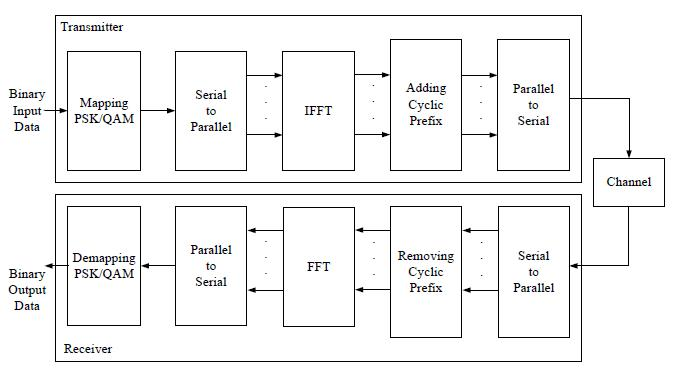
\includegraphics[width=12cm]{content/fig/basic_ofdm_design.JPG}
\label{fig:basic_ofdm}
\captionof{figure}{Basic baseband OFDM system}
\end{center}

In practice, to prevent sharp transactions at the sample time boundaries, a windowing block is used for filter shaping. In conclusion, spectrum utilization is enhanced dramatically. Therefore, the baseband OFDM symbol can be written as below:\\
\begin{equation} \label{ofdm_window}
\begin{split}
s_{k}(t)=
\left\{
	\begin{array}{ll}
	w(t - t_{s})\sum\limits_{i=-\frac{N}{2}}^{\frac{N}{2}-1} d_{i+\frac{N}{2}} \exp\lbrack j2\pi\frac{i}{T}(t- t_{s}- T{g}) , & t_{s}\le t < t_{s} + (1+\beta)T_{sym}\\
	0, & \mbox{otherwise}
	\end{array}
\right.
\end{split}
\end{equation}

where $T_{g}$ is the guard interval duration, $T_{sym}= T+ T_{g}$ is the OFDM symbol period,
symbol starting time $t_{s}= kT_{sym}$, and $w(t-t_{s})$ is the pulse shaping window, which is
usually a raised cosine filter, and $\beta$ is the roll-off factor.\\
The OFDM mechanism is used in 802.11 and Wimax standards. It has good tolerance against multipath and the receiver is easier to implement. We will see the details of implementations in practical systems.\\


\section{OFDM Specifications in IEEE 802.11a Standard}

\subsection{Introduction of IEEE 802.11}
The Institute of Electronic and Electrical Engineers (IEEE) has released IEEE 802.11 in June 1997. The standard defined physical and MAC layers of wireless local area networks (WLANs).\\
The physical layer of the original 802.11 standardized three wireless data exchange techniques:

\begin{itemize}
  \item Infrared (IR);
  \item Frequency hopping spread spectrum (FHSS);
  \item Direct sequence spread spectrum (DSSS).
\end{itemize}


The 802.11 radio WLANs operate in the $2.4 GHz$ ($2.4$ to $2.483 GHz$) unlicensed Radio Frequency (RF) band. The maximum isotropic transmission power in this band allowed by FCC in US is $1 Wt$, but 802.11 devices are usually limited to the $100 mWt$ value.

The physical layer in 802.11 is split into Physical Layer Convergence Protocol (PLCP) and the Physical Medium Dependent (PMD) sub layers. The PLCP prepares/parses data units transmitted/received using various 802.11 media access techniques. The PMD performs the data transmission/reception and modulation/demodulation directly accessing air under the guidance of the PLCP. The 802.11 MAC layer to the great extend is affected by the nature of the media. For example, it implements a relatively complex for the second layer fragmentation of PDUs.\\

\begin{center}
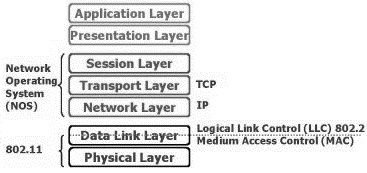
\includegraphics{content/fig/osi.JPG}
\captionof{figure}{OSI Reference Model.}
\end{center}

\subsection{System Design}

In reality, having an anti-aliasing configuration, oversampling is performed before passing the digital signal to digital-to-analog converter. There are many other blocks in standards like channel coding, symbol interleaving and channel estimation.\\
In comparison to the fundamental architecture shown in Figure 000, some other building blocks are added in a practical IEEE 802.11 design shown in Fig 00, marked with blue and dashed on line. At the transmitter, several "null" subcarriers or tones are reserved besides of the data subcarriers in order to perform oversampling of the transmitted signal. In this context, "null" means the symbol carried on this subcarrier has a value of zero. Besides, some other subcarriers used as pilot for channel estimation are also inserted. The subcarriers are allocated at the input of the IFFT block to generate a phase shift. The windowing for pulse shaping is achieved after CP extension.\\

\begin{center}
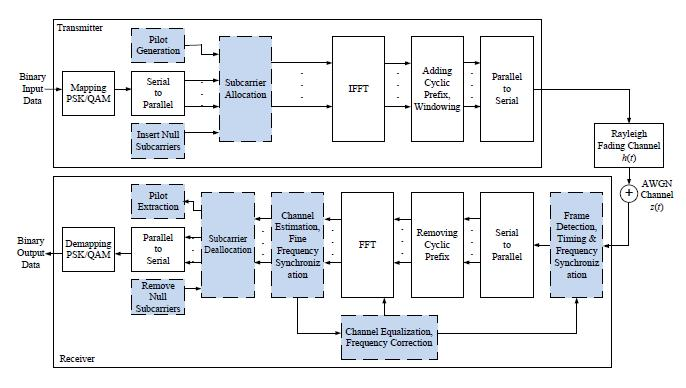
\includegraphics[width=12cm]{content/fig/ieee_system_design.JPG}
\captionof{figure}{Architecture of an OFDM system}
\end{center}

At the receiver side, the frame synchronization and detection for both timing and frequency is performed in the first stage. Channel estimation is performed after the FFT block outputs the preambles in the frequency domain. The result is fed back to the FFT block for the equalization, which eliminates the effects of fading channel, while the fine synchronization for both timing and frequency is also added to further improve the system performance.\\
At least these basic parameters should be specified for a system design:

\begin{enumerate}
  \item Delay spread expected for the channel ($300 ns$)
  \item Guard duration ($800 ns$) which describes symbol duration ($4.0 \mu s$)
  \item Available bandwidth
  \item Data rate
\end{enumerate}

For indoor environment a delay spread less than 300 ns expected. We consider the guard duration 800 ns, which effectively protects the signal from ISI in the indoor environment and some of the outdoor wireless communication environments. Five times the guard duration for limiting the power and bandwidth loss is regarded for the symbol duration, and is set to 4.0 $\mu$s in our case. Hence, the OFDM symbol rate is 0.25 mega symbol per second (Mbaud).\\
Keep in mind, the useful OFDM symbol duration without the guard interval is 3.2 $\mu$s. So, the subcarrier spacing, which is the reciprocal of the useful symbol duration, can be determined as 312.5 kHz. Assuming that there is a bandwidth of 20 MHz available, the number of subcarriers is calculated to be 64. This is exactly the same as the specification defined in IEEE 802.11a standard.\\
As mentioned, some tones are reseved for pilot subcarries (channel estimation), null subcarriers (realizing oversampling to avoid aliasing) and windowing (reduce the out-of-band spectral energy).\\
In our design we chose 48 data tones and 4 pilot subcarriers. So, 52 subcarries are occupied. Applying a raised-cosine window with roll-off factor $\beta$= 0.02 the total occupied bandwidth is\\

\begin{equation} \label{occupied_bw}
(1+ 0.02)\times(52 \times 312.5kHz) \approx 16.6MHz
\end{equation}

To accomplish Oversampling, some zeros before and after the data vector are appended in the frequency domain as shown below.\\

\begin{equation} \label{over_sample}
\overbrace{0, 0, ... , 0,}^{1/2\;appended\;zeros}
\underbrace{d_{-\frac{N_d}{2}}, d_{-\frac{N_d}{2}+1}, ... , d_{-1},}_{Negative\;subcarriers}
\underbrace{d_{1}, d_{2}, ... , d_{\frac{N_d}{2}},}_{Positive\;subcarriers}
\overbrace{0, 0, ... , 0}^{1/2\;appended\;zeros}
\end{equation}

In the IEEE 802.11a transmitter, a 64 point IFFT multiplexes the orthogonal sub-carriers and the sub-carriers are renumbered as in Figure \ref{freq_alloc} before performing the Fourier transformation. Only 48 of them are used for data transmission and they are modulated by using BPSK, QPSK, 16-QAM or 64-QAM according to the Rate parameter. The sub-carriers $P_{-21}$, $P_{-7}$, $P_{7}$ and $P_{21}$ are dedicated to comb-type pilot signals which are used to track the phase variations due to the time varying channel or a frequency o set error. The pilot sub-carriers are modulated by using BPSK and to prevent the generation of spectral lines, they transmit a pseudo random binary sequence generated by the same polynomial used in the scrambler.\\

\begin{center}
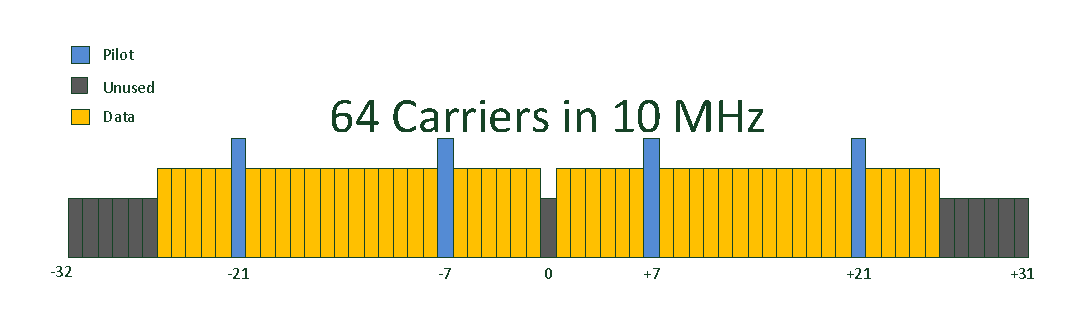
\includegraphics[width=\textwidth]{content/fig/freq_alloc.JPG}
\captionof{figure}{The frequency allocation of IEEE 802.11a sub-carriers}
\label{freq_alloc}
\end{center}

The nonzero data values are mapped onto the subcarriers around 0 Hz, and the zeros are mapped onto frequencies around sampling rate.
Basically, in the BPSK modulation is applied on each subcarrier, each symbol for an individual subcarrier has one bits. The bit rate achieves without channel coding:\\

\begin{equation} \label{bitrate_achiv}
\frac{1}{4.0\mu s} \times 48 \times 1= 12Mbps
\end{equation}

The same calculation can be perform for QPSK to reach 24Mbps. But, channel coding will reduce this values. Variation of coding rates and modulation methods, In the 802.11a standard, the data rate ranges from 6 Mbps to 54 Mbps.\\

\begin{center}
\captionof{table}{System parameters defined for the proposed OFDM system}
\label{table:sys_param}
\vspace{0.5cm}
\begin{tabular}{c|c|c}
Parameter&Description&Value\\ \hline
$B_{w}$&Available channel bandwidth&$20MHz$\\
$\sigma_{\tau}$&Delay spread of the channel& $<300 ns$\\
$T_{g}$&Guard interval duration (Cyclic Prefix)&$0.8\mu s$\\
$T_{sym}$&OFDM symbol period&$4.0\mu$\\
$T$&Effective symbol duration (FFT period)&$3.2\mu s (=T_{g}- T_{sym})$\\
$\Delta f$&Subcarrier spacing&$312.5kHz (=1/T)$\\
$N_{g}$&Number of guard samples&$16$\\
$N$&FFT size&$64= B/\Delta f s$\\
$N_{d}$&Number of data subcarriers&$48$\\
$N_{p}$&Number of pilot sucarriers&$4$\\
$N_{u}$&Number of used subcarriers&$52$\\
$B_{u}$&Signal occupied bandwidth&$16.6MHz$\\
&Modulation type&$BPSK, QPSK$\\
$R_{b}$&Data rate without coding&$12Mbps, 24Mbps$\\
\end{tabular}
\end{center}

Table \ref{table:code_vs_rate} shows the length parameter indicates the number of information bytes with different code rates:

\begin{center}
\captionof{table}{Rate dependant parameters in IEEE 802.11a Standard}
\label{table:code_vs_rate}
\vspace{0.5cm}
\begin{tabular}{c|c|c|c|c}
Data rate&Modulation&Code Rate&Coded bits per symbol&Data bits per symbol\\ \hline
6 Mbps&BPSK&1/2&48&24\\
9 Mbps&BPSK&3/4&48&36\\
12 Mbps&QPSK&1/2&96&48\\
18 Mbps&QPSK&3/4&96&72\\
24 Mbps&16QAM&1/2&192&96\\
36 Mbps&16QAM&3/4&192&144\\
\end{tabular}
\end{center}

The theoretical equation of the Bit-Error Rate for a QPSK channel is:\\

\begin{equation} \label{theo_ber}
P_{b}(e)= \dfrac{1}{2}erfc(\sqrt{\dfrac{E_{b}}{N_{0}}})
\end{equation}

It is discussed that the BER can be computed by considering the non-ideality which the two parameters \textit{guard time} and \textit{pilots} will inject into the result. The formulation would be:\\

\begin{equation} \label{theo_ber_guard_pilot}
P_{b}(e)= \dfrac{1}{2}erfc(\sqrt{\dfrac{E_{b}}{N_{0}}\dfrac{T}{T+T_{g}}\dfrac{N_{u}}{N_{u}+N_{p}}})
\end{equation}

Replacing the standard value from Table \ref{table:sys_param} in the equation we have:\\

\begin{equation} \label{theo_ber_ieee}
P_{b}(e)= \dfrac{1}{2}erfc(\sqrt{\dfrac{E_{b}}{N_{0}}0.65})
\end{equation}

\subsection{IEEE 802.11a Standard in Time and Frequency}
A packet of OFDM will be described here. In an OFDM frame, a preamble which carries no data is transmitted first, followed by the signal field which give some information about data and transmitted data. As indicated in Figure 00, an OFDM frame has the general form as below:
\begin{equation} \label{sym_ofdm}
s_{OFDM}(t)= s_{preamble}(t)+ s_{signal}(t- T_{preamble})+ s_{data}(t- T_{preamble}- T_{signal})
\end{equation}

where\\
\begin{equation} \label{preamble_ofdm}
s_{preamble}(t)= s_{short}(t)+ s_{long}(t- T_{short})
\end{equation}

As shown in Figure \ref{preamble_ieee}, the preamble starts with 10 short training symbols (STSs) from $T_{1}$ to $T_{10}$, followed by a guard interval ($GI_{2}$) and two long training symbols (LTSs) $L_{1}$ and $L_{2}$. Both the short and long training sequences have an $8 \mu s$ duration and the entire preamble lasts for $16 \mu s$. Then, a $3.2 \mu s$ signal symbol, as well as 800 ns guard interval is transmitted. This field bears some information necessary for the data symbols, such as the coding rate and length. Finally the various data symbols that carry user information are transmitted. Each data symbol has a duration of $4.0 \mu s$, within which there is a 800 ns CP, as already described.\\
The application of STS and LTS for training are different. STS used for AGC, frame detection, coarse timing and frequency synchronization. Each symbol in this sequence has a duration of 800 ns and contains 16 samples, and is identical to one another.
 It will be shown in a professional system, auto-correlation will apply to this portion to perform such the operations. After the short training sequence is transmitted, a $1.6 \mu s$ guard interval that contains 32 samples is introduced. The LTS is cyclically extended within this interval. Then two identical LTSs with the same duration of $4.0 \mu s$ are followed. The LTS is used for fine frequency offset and channel estimation. It will be described that a cross-correlation with a stored array is done for extraction of the offset.\\
The data being transmitted should pass several stages and be prepared by PLCP (Physical Layer Convergence Procedure) before transmission. The preamble and the PLCP header are transmitted at 1Mbps regardless of the current data transmission speed. After the preamble the payload prepared by the MAC layer is sent to the receiver at the rate specified in the services field.\\
The picture below shows the OFDM packet data layout. It starts with training sequence (PLCP preamble), followed by the SIGNAL field and data. The data is followed by 6 tail bits and padding (not shown on the picture). Both the training sequence and the 24 bit SIGNAL field are transmitted at $6 Mbps$ rate. The SIGNAL field tells the receiver at what rate the following data will be transmitted and indirectly defines the subcarriers' modulation technique employed. The BPSK, QPSK, 16-QAM and 64-QAM are the available choices. The SIGNAL field also delivers the length (12 bit) of the following data and includes a zero bit sequence for the data scrambler synchronization. The total training sequence and SIGNAL field transmission times add up to about $20 \mu s$, which is an overhead equivalent to approximately 140 bytes transmission at the maximum transmission rate of 54Mbps defined by the standard.\\

\begin{center}
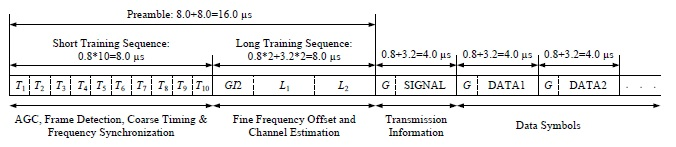
\includegraphics[width=12cm]{content/fig/ofdm_frame.JPG}
\captionof{figure}{Preamble of IEEE 802.11}
\label{preamble_ieee}
\end{center}

As we already analyzed, 52 subcarriers are used for an OFDM data symbol and pilot. Oversampling is achieved by adding 12 null subcarriers in order to eliminate aliasing which might occur during digital to analog conversion. Because FFT shift is performed, the null subcarriers with a value of zero are located in the middle of the input vector for the IFFT block. Note that dc carrier is not used to transmit data. The short and long training sequences can also be applied to this mapping rule, since they both have a length of 52 samples with frequency index from -26 to +26.\\


\subsection{Origin of CFO}
A simple model of a radio transmitter and receiver can depict the basis of the CFO source.

\begin{center}
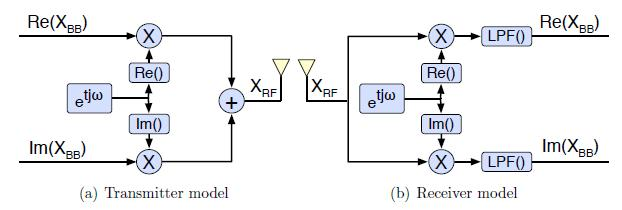
\includegraphics[width=\textwidth]{content/fig/cfo_radio_model.JPG}
\captionof{figure}{General models of a direct conversion RF}
\label{cfo_radio_model}
\end{center}

In Figure \ref{cfo_radio_model}, $\omega$ is The carrier frequency and $X_{BB}$ is the complex baseband signal, $X_{RF}$ is
a real-valued RF signal. These models simplified many other operations in a real RF transceivers although none of these affect the up/down-conversion processes as they relate to CFO.\\
These equations about transmit and receive processes can be written in equation (\ref{eq_tx_rx_process}):

\begin{equation}\label{eq_tx_rx_process}
\begin{split}
X_{RF} & = TX(X_{BB})\\
& = Re(X_{BB})\cos(\omega t) - Im(X_{BB})\sin(\omega t)\\
& = \frac{1}{2} (X_{BB} e^{jt\omega} + X^{*}_{BB} e^{-jt\omega})\\
\\
X_{BB} & = RX(X_{RF}, \omega)\\
& = LPF(X_{RF} e^{j\omega t})
\end{split}
\end{equation}


Assume a signal $S_{BB}$ transmitted with carrier frequency $\omega_{S}$ which is received with carrier frequency $\omega_{D}$. we can express the received baseband signal $D_{BB}$ in terms of the transmitted baseband signal $S_{BB}$ and the carrier frequencies. Then:\\

\begin{equation} \label{DBB_SBB}
\begin{split}
D_{BB} & = LPF(\frac{(S_{BB} e^{jt\omega_{S}} + S^{*}_{BB} e^{-jt\omega_{S}})e^{jt\omega_{D}}}{2})\\
&= S_{BB}(e^{jt(\omega_{S}- \omega_{D})})
\end{split}
\end{equation}

The received baseband signal is equal to the original baseband signal modulated by a complex sinusoid. In the frequency domain, this gives a received spectrum equal to the transmitted one, only shifted away from DC by the difference in the carrier frequencies of the transmitter and receiver (i.e. $\omega_{S}- \omega_{D}$). This shift of the received
signal is the baseband manifestation of carrier frequency offset.

\subsection{Impact of CFO}
\label{Impact_of_CFO}
There are two destructive impacts on an OFDM system. Firstly, the phase offset across subcarriers in an symbol which can be  estimated and corrected in frequency domain to prevent errors in a constant rotated constellation. Some subcarriers are allocated as pilot tones which receiver can estimate phase errors.\\
The second effect of CFO is the degradation of orthogonality between subcarriers in receiver's FFT which causes inter-carrier interference (ICI). ICI acts an effective SNR reduction as a result of CFO increasing. [...]\\
The impact is displayed in Figure \ref{cfo_impact_on_ici} which is shown simulated OFDM system uses 10 MHz bandwidth and 64 subcarriers, 48 of on a random 16-QAM data symbols. CFO and AWGN are applied between the transmitter and receiver. The receiver model uses perfect knowledge of the CFO to correct the phase offset in each OFDM symbol, but does not implement any correction for ICI.\\

\begin{center}
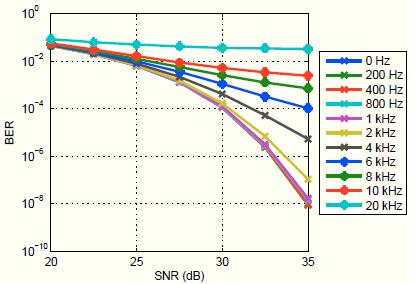
\includegraphics[width=10cm]{content/fig/cfo_on_ici.JPG}
\captionof{figure}{OFDM performance loss due to CFO-induced ICI.}
\label{cfo_impact_on_ici}
\end{center}

The results shows that for large CFOs errors caused by ICI dominate performance, even at high SNR. It is also
clear that for small CFOs performance is dominated by SNR. Specifically, for frequency offsets smaller than 1 kHz, the
performance degradation due to ICI is negligible.\\
Let's focus on LTS part in a OFDM symbol, Figure \ref{sym_ofdm}, for a while. In time domain, we have 160 samples in this section which creates to complete LTS symbols and a half. Each LTS symbol has 64 samples shown in Figure \ref{lts_time_domain}.\\

\begin{center}
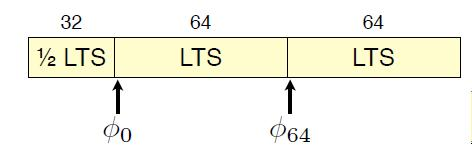
\includegraphics[width=10cm]{content/fig/LTS_time_domain.JPG}
\captionof{figure}{LTS in Time Domain.}
\label{lts_time_domain}
\end{center}

We can say:
\begin{equation} \label{cfo_cal}
\begin{split}
CFO \approx (\phi_{64}- \phi_{0})\\
CFO_{EST} = \frac{f_{s}}{2\pi . 64^{2}} \sum\limits_{n=64}^{127} \phi_{n}- \phi_{(n-64)}\\
\end{split}
\end{equation}


\begin{center}
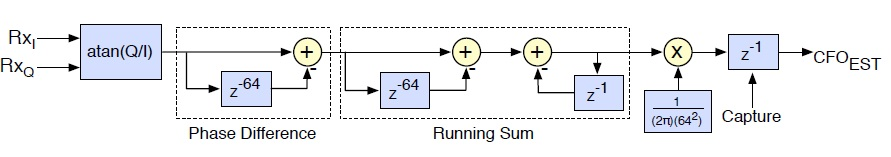
\includegraphics[width=\textwidth]{content/fig/cfo_est.JPG}
\captionof{figure}{Time Domain CFO Estimation.}
\label{cfo_est}
\end{center}

Which $CFO_{EST}$ is the estimated CFO. To have such the structure in the Simulink we can arrange as Figure \ref{cfo_est}.
\begin{abstract}
An OFDM structure from modulator to demodulator is studied. The aim is to investigate the characteristics of the system in different conditions and comparing the behavior with the single carrier configuration. The simulation conditions change in the cyclic prefix size, a Non-Linear Amplifier (NLA), multipath and equalizer activation. \\ Optimization on the cost function for the system is done. Semi-Analysis calculation for noise for a target Bit Error Rate (BER) of $10^{-3}$ are done. OFDM simulation is based on the characteristic of Fast Fourier Transform.\\
The analysis shows that using a multipath increases the needed \textit{energy per bit to noise power spectral density ratio} $(E_{b}/N_{0})$ by $13dB$ in order to reach the target BER when the NLA block is deactivated. An equalization block improves by $8dB$ the $(E_{b}/N_{0})$. In comparison, the multipath, more than the guard time of the signal, does not influence the BER so much.\\ With activated NLA with fixed $\beta=10$ the $E_{b}/N_{0}$ has to be amplified by almost $0.8dB$ in order to reach the target BER. \\ The optimized back-off of $\beta=8$ improves this value by $14dB$ when equalization block is activated.
 
\end{abstract}

\section{Introduction}
An OFDM communication system is simulated. Different characteristics of the system are examined and parameters are adjusted to study.\\ A block based signaling configuration is chosen for the implementation. As a result, the realization of the modulator is done thanks to IFFT computation characteristics. Cyclic prefixes are added to the resulting OFDM symbols as well as guard time filling. On the demodulator an FFT block recreates the initial input of the system. \\
An optimization is performed on the input back-off of a Non-Linear Amplifier (NLA). The back-off of the NLA is normally more than in a single carrier system because of better performance of the inter symbol interference (ISI) thanks to smaller coherent bandwidth which let us work on less power. \\
A description of the the system is given in section \ref{sec_systemmodel}. Section \ref{sec_simstruct} describes the varied parameters and analysis values while in section \ref{sec_anasim} observations on the simulation are presented and characteristics of the system are shown. Before the conclusion in section \ref{sec_conclusion}, section \ref{sec_optimization} describes the optimization of the system.

\section{System Model}
\label{sec_systemmodel}
\begin{figure}[tbp]
\centering
\includegraphics[width=\textwidth]{content/fig6/ofdmmodel1.JPG}
\includegraphics[width=\textwidth]{content/fig6/ofdmmodel2.JPG}
\caption{OFDM System Model}
\label{fig_ofdmsystemmodel}
\end{figure}

Figure \ref{fig_ofdmsystemmodel} presents the OFDM system block diagram.
Basic steps of the praxis are realized in blocks in the simulation. Additionally is shown how the composition of data changes in the single steps of the system.\\
The first block represents the data source. They are the bits which an application may send. In the simulation it is realized by a random bit generator. The following QPSK modulation block converts this bits into symbols, which are complex numbers. Each symbol carries several bits. The third block is the first one actually relevant for OFDM. The serial symbol stream is converted into a channel and OFDM symbol structure. In the simulation it is represented in a matrix shape where the rows are different channels and each column is an OFDM symbol. This means that each OFDM symbol, formed by $c$ (\#channels) serial symbols (complex numbers), is distributed over the $c$ channels.\\
In the next step zero channels are added in order to separate well subsequent OFDM symbols. For the simulation structure zero rows are added in the middle of the matrix. The following block interprets each symbol (complex number) of an OFDM symbol as a orthogonal frequency and converts each OFDM symbol per IFFT into a vector of time discrete values of the same length. As sixth step the cyclic prefix insertion is done. In order to maintain orthogonality of the frequencies but prevent ISI, an amount of \textit{guard values} are copied from the end of each OFDM symbol to its beginning. The number of rows in the simulation matrix grows by that by the number of \textit{guard values}.\\
The following block is the NLA which depends on the optimization parameter $\beta$ (back-off). At this point the transmitter side ends. In order to simulate the multipath a convolution is made on each OFDM symbol with the delay filter. Since the simulation is made on each OFDM symbol separated, this operation works with a memory in order simulate a serial transmission.\\
The receiver side is just the opposite of the transmitter. In the cyclic prefix remover the copied values are deleted and the simulation matrix size decreases. The next block performs the FFT on each OFDM symbol which reconstructs the as frequencies interpreted complex numbers.\\ The following equalization block tries to remove the effect of the multipath. For the simulation a multiplication with the inverted transfer function of the multipath is operated. By this, only the phase of the complex symbols changes.\\ Finally, the zero channels are removed and the matrix structure is reconverted to a series of symbols. The following analysis is done on the received symbols and consequently they are not demodulated into a bitstream.

\section{Simulation Structure}
\label{sec_simstruct}
Fundamentally, we do block-by-block simulation thanks to IFFT for parallel processing. Simulation is done by (de)activation of the blocks on Figure \ref{fig_ofdmsystemmodel}.
First, we study the noise semi-analysis by having only the basic blocks activated and also to examine the correctness of them. The basic blocks for our OFDM system are IFFT and FFT, Cyclic addition and removal and the semi-analyzer block. 
The theoretical equation of the BER for a QPSK channel is:\\
\begin{center} 
$P_{b}(e)= \frac{1}{2}erfc(\sqrt{\frac{E_{b}}{N_{0}}})$\\
\end{center}
It is discussed that the BER can be computed by considering the non-ideality which the two parameters \textit{guard time} and \textit{pilots} will inject into the result. The formulation would be:\\
\begin{center}
 $P_{b}(e)= \frac{1}{2}erfc(\sqrt{\frac{E_{b}}{N_{0}}\frac{T}{T+T_{g}}\frac{N_{u}}{N_{u}+N_{p}}})$\\
\end{center}

In the next step, the NLA block is activated and its effect is studied. We have chosen NLA number 3 and try to optimize its back-off.
Later, the channel impulse response modeled by considering two multipaths with different delays is implemented by an FIR filter. This extended simulation will be compared with NLA in the scenario and also the equalizer. Finally, we optimize the system by adjusting the back-off parameter of NLA in an AWGN channel.\\
When we study the equalization block we consider such equation for the received tones:
\begin{center}
$y_{i}= H_{i} \lambda_{i} + n_{i}$\\
\end{center}
Without equalization the BER would be:
\begin{center}
$P_{b}(e)= \frac{1}{2}erfc(\frac{H_{i} \lambda_{i}}{\sqrt{2 \sigma^{2}}})$\\
\end{center}
Then, after the equalization, the formula will be changed to this:\\
\begin{center}
$y^{\prime}_{i}= \lambda_{i} + \frac{n_{i}}{H_{i}}$\\
\end{center}
and the BER to
\begin{center}
 $P_{b}(e)= \frac{1}{2}erfc(\frac{\lambda_{i}}{\sqrt{2 \sigma^{2}}})$\\
\end{center}
and NOT: $P_{b}(e)= \frac{1}{2}erfc(\frac{\lambda_{i}}{\sqrt{\frac{2 \sigma^{2}}{H_{i}}}})$, as it may be guessed wrongly. The power spectral density of the noise is not decreased.
\section{System Design in System Generator}
\label{sec_anasim}

\begin{center}
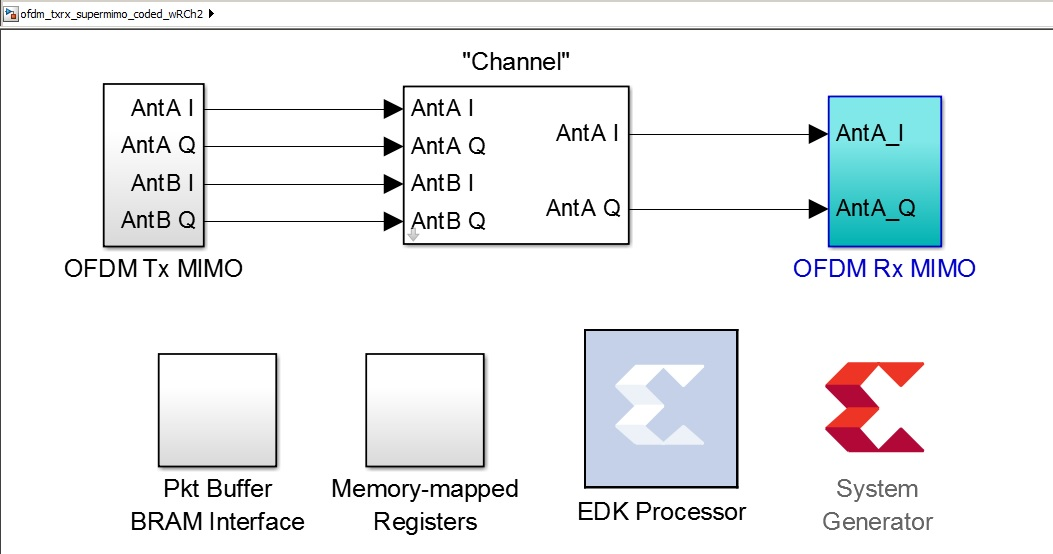
\includegraphics[width=\textwidth]{content/fig/system.JPG}
\captionof{figure}{OFDM System.}
\label{ofdm_system}
\end{center}


\begin{center}
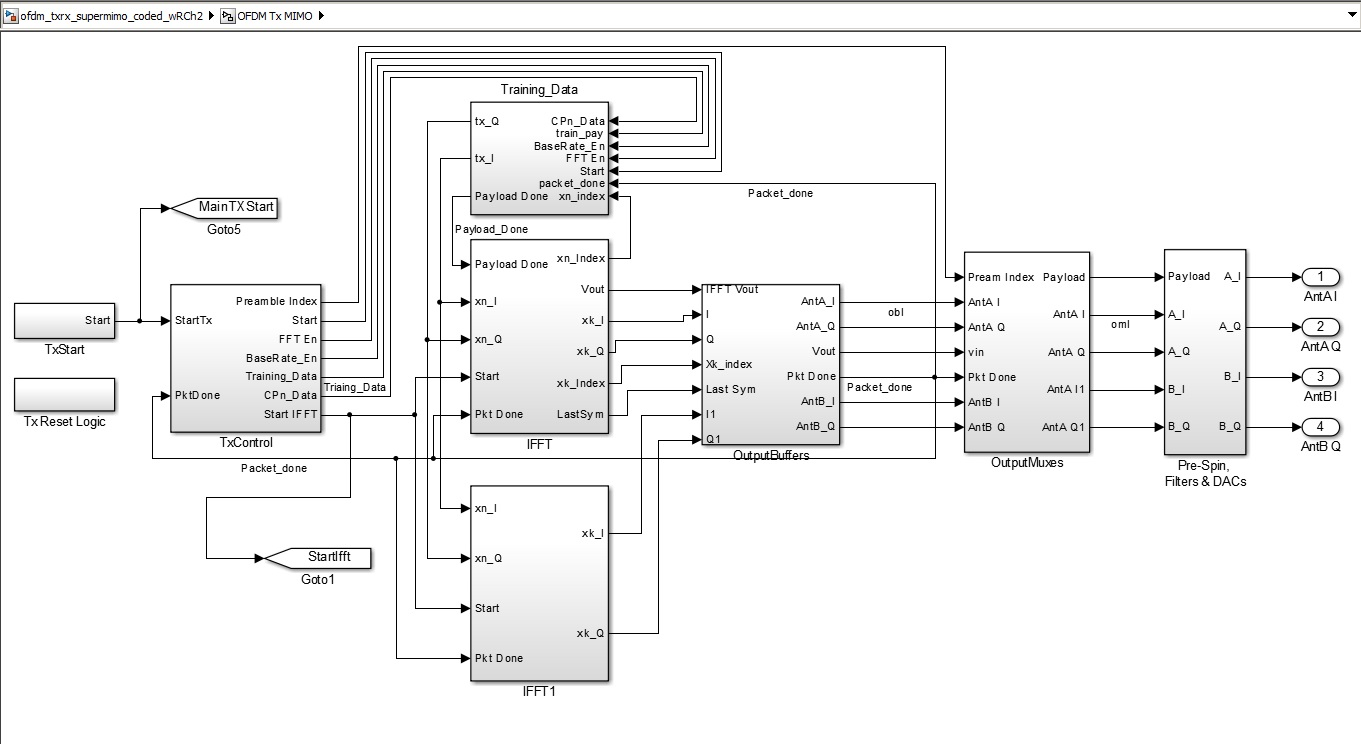
\includegraphics[width=\textwidth]{content/fig/txblock.JPG}
\captionof{figure}{OFDM Transmitter Block.}
\label{tx_block}
\end{center}

\begin{center}
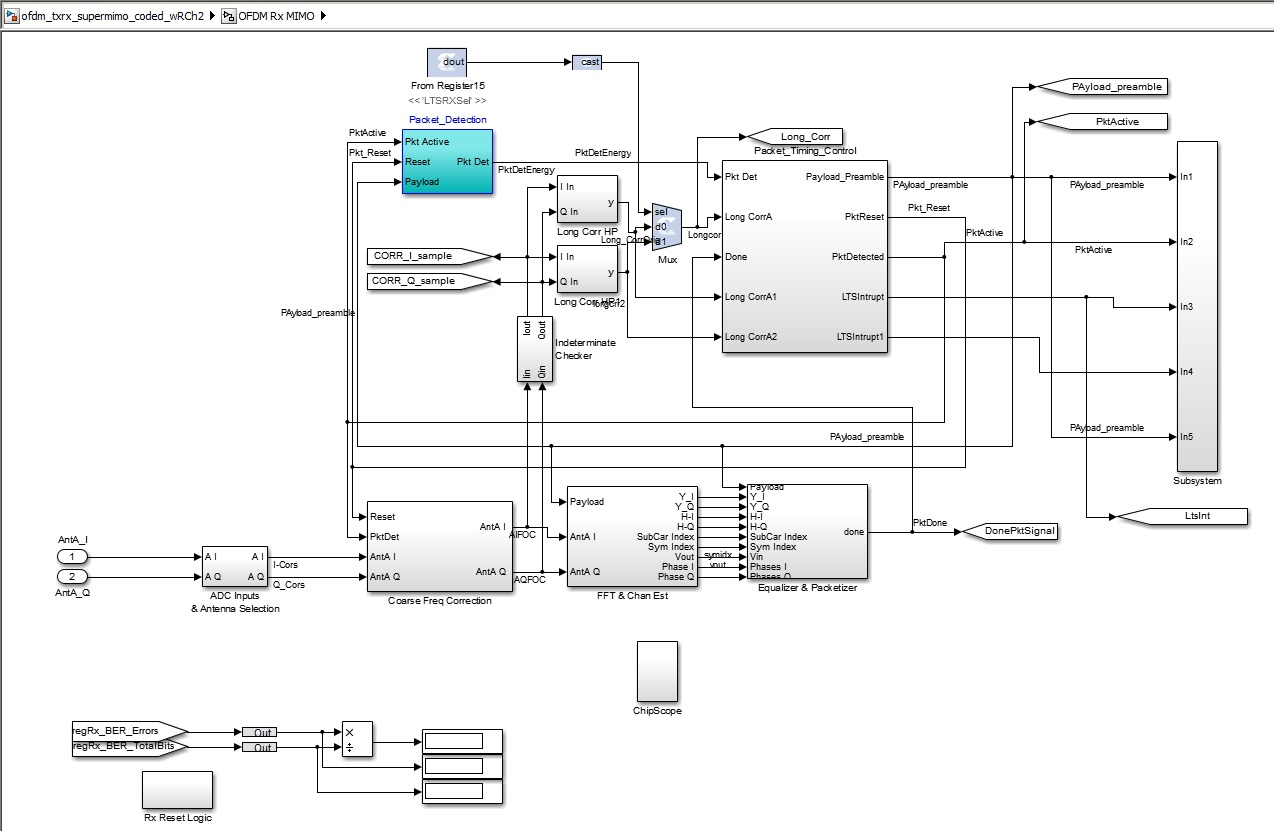
\includegraphics[width=\textwidth]{content/fig/rxblock.JPG}
\captionof{figure}{OFDM Receiver Block.}
\label{rx_block}
\end{center}

\begin{center}
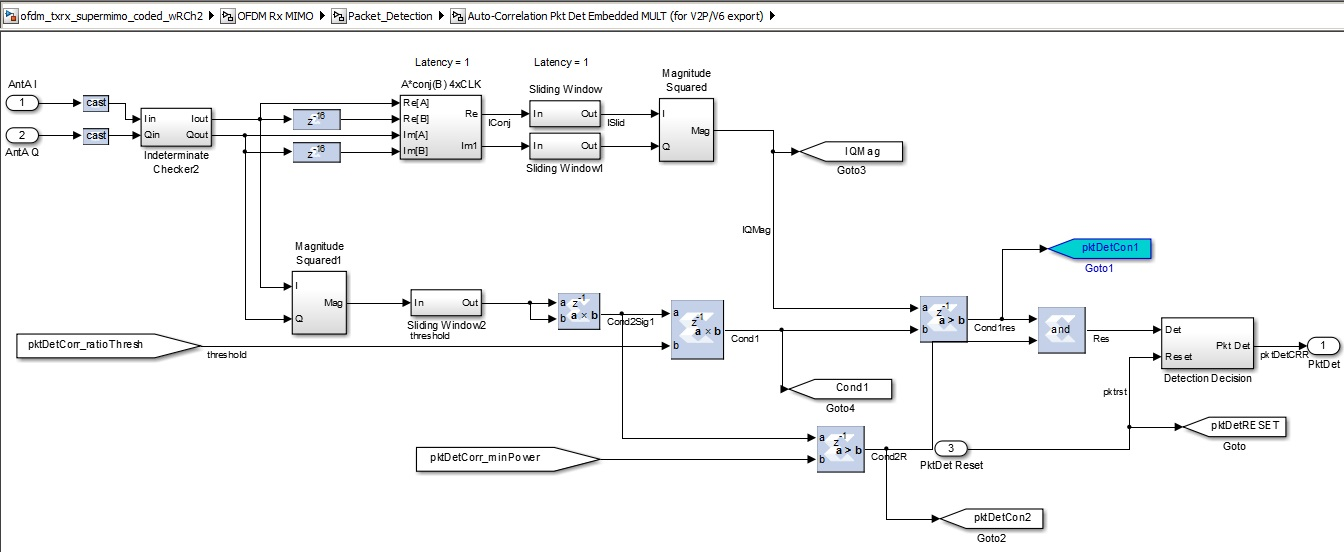
\includegraphics[width=\textwidth]{content/fig/autocorrblock.JPG}
\captionof{figure}{Auto-Correlation Block.}
\label{autocorrblock}
\end{center}

\begin{center}
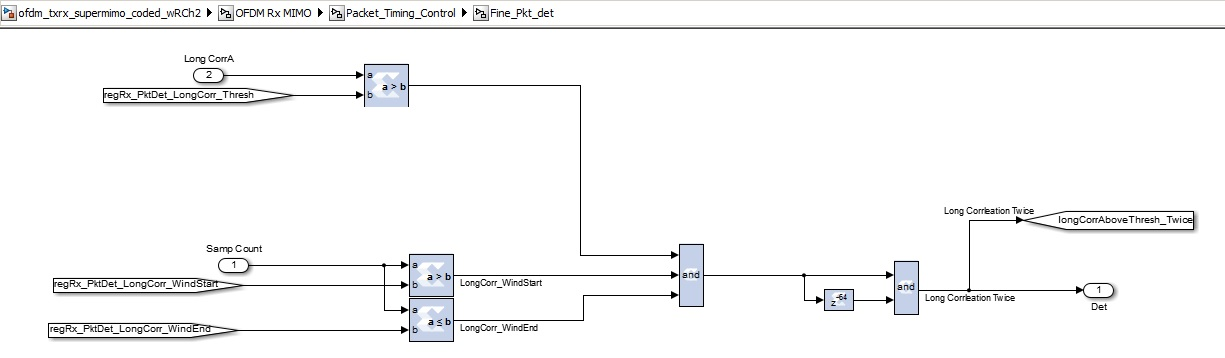
\includegraphics[width=\textwidth]{content/fig/fine_packetDetect.JPG}
\captionof{figure}{Fine Packet Detection Block.}
\label{autocorrblock}
\end{center}

\section{Hardware Samples and Analysis}
\label{hw_samples}

\begin{center}
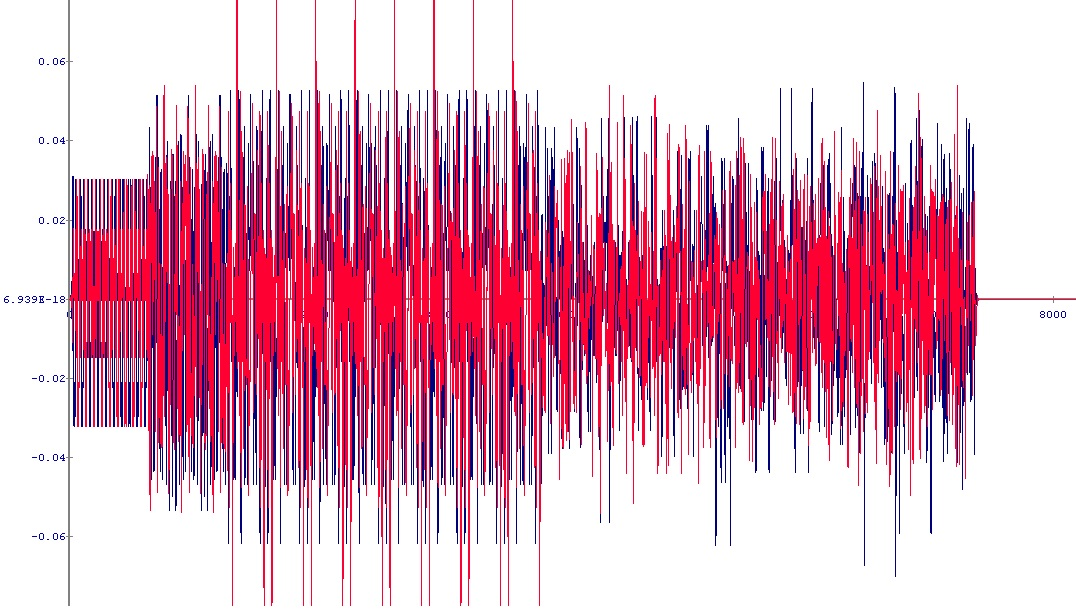
\includegraphics[width=\textwidth]{content/fig/ofdmframe_chipscope.JPG}
\captionof{figure}{OFDM Frame (I/Q) detected in Chipscope.}
\label{ofdmframe_chipscope}
\end{center}

\begin{center}
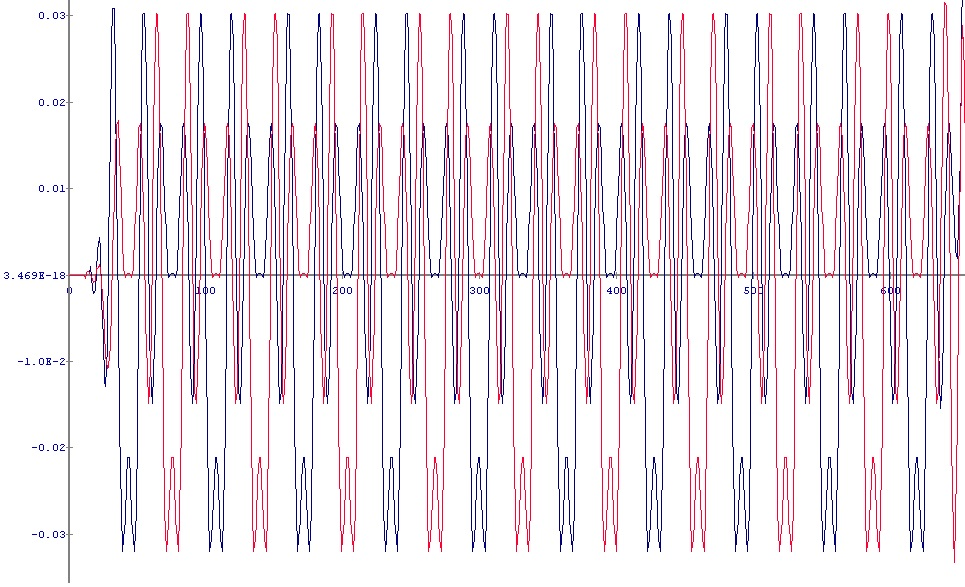
\includegraphics[width=\textwidth]{content/fig/sts_chipscope.JPG}
\captionof{figure}{STS (I/Q) detected in Chipscope.}
\label{sts_chipscope}
\end{center}

\begin{center}
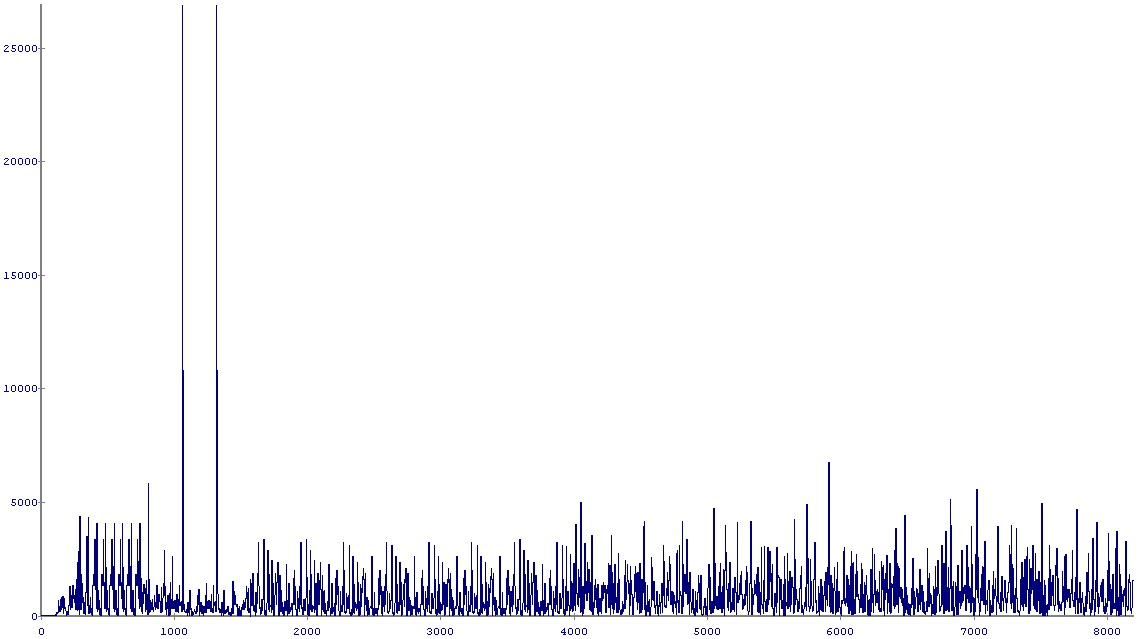
\includegraphics[width=\textwidth]{content/fig/crosscorr.JPG}
\captionof{figure}{Cross-Correlation detected in Chipscope.}
\label{crosscorr}
\end{center}


\begin{center}
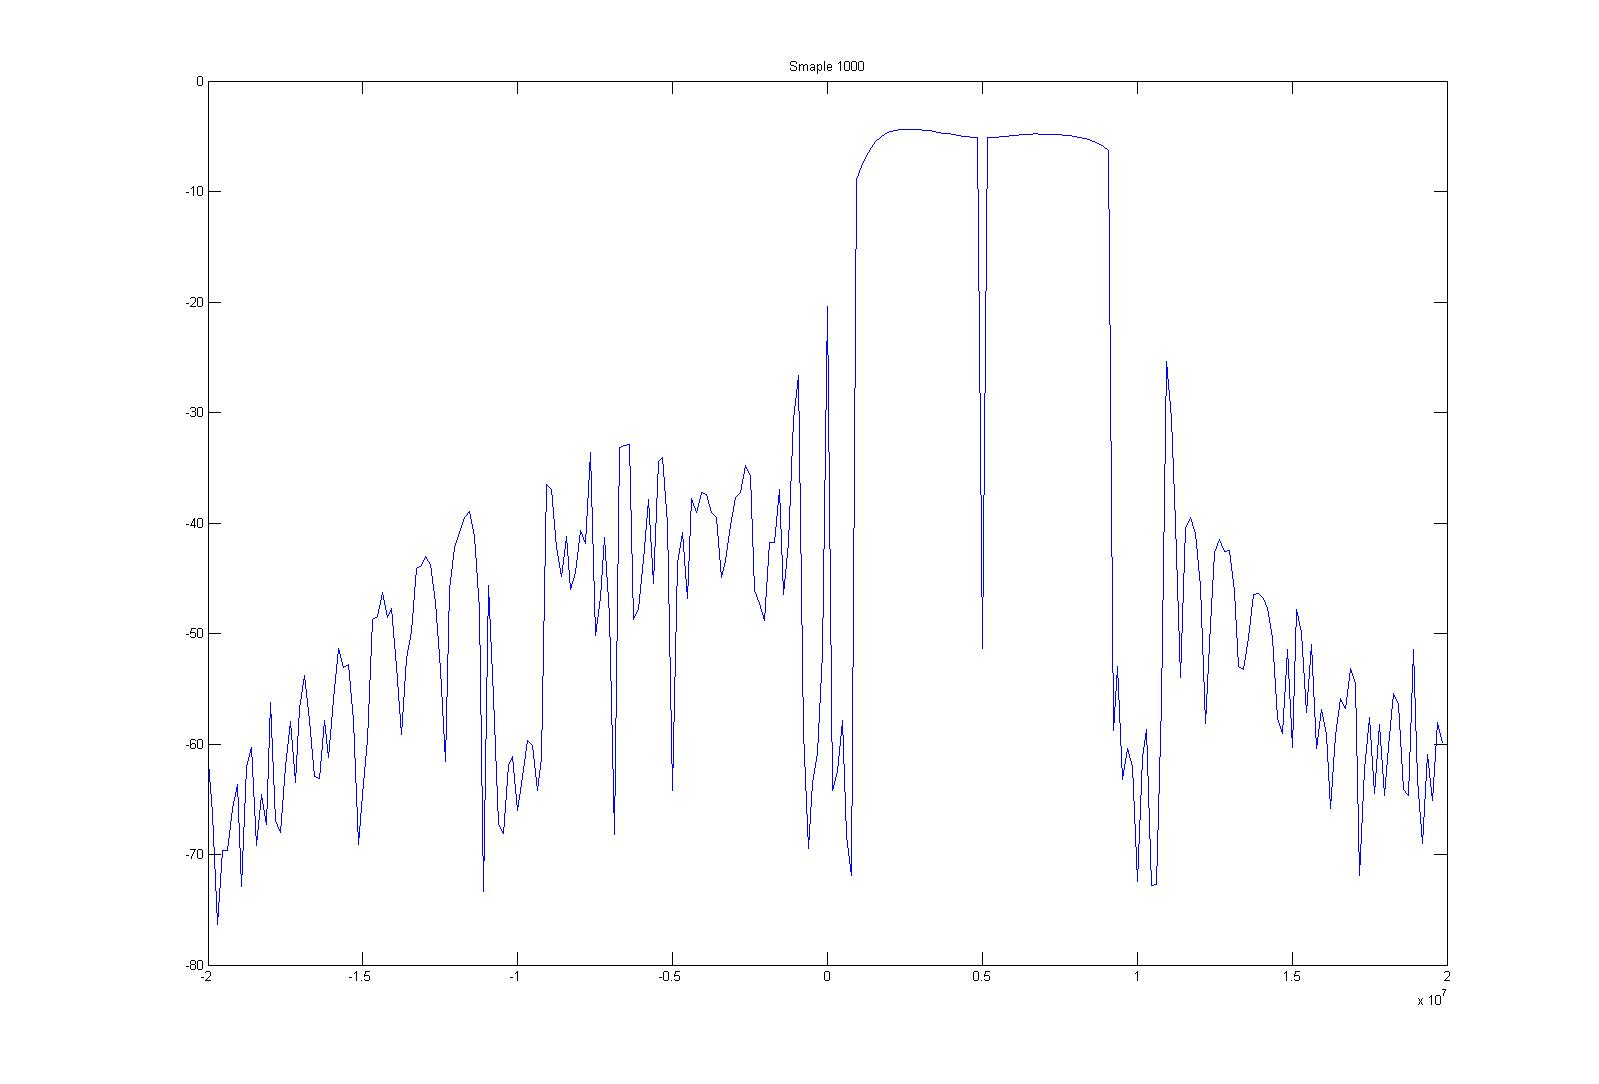
\includegraphics[width=\textwidth]{content/fig/baseIFAdcDac.JPG}
\captionof{figure}{LTS Spectrum in Baseband chain (IF filter is enable)}
\label{baseIFAdcDac}
\end{center}

\begin{center}
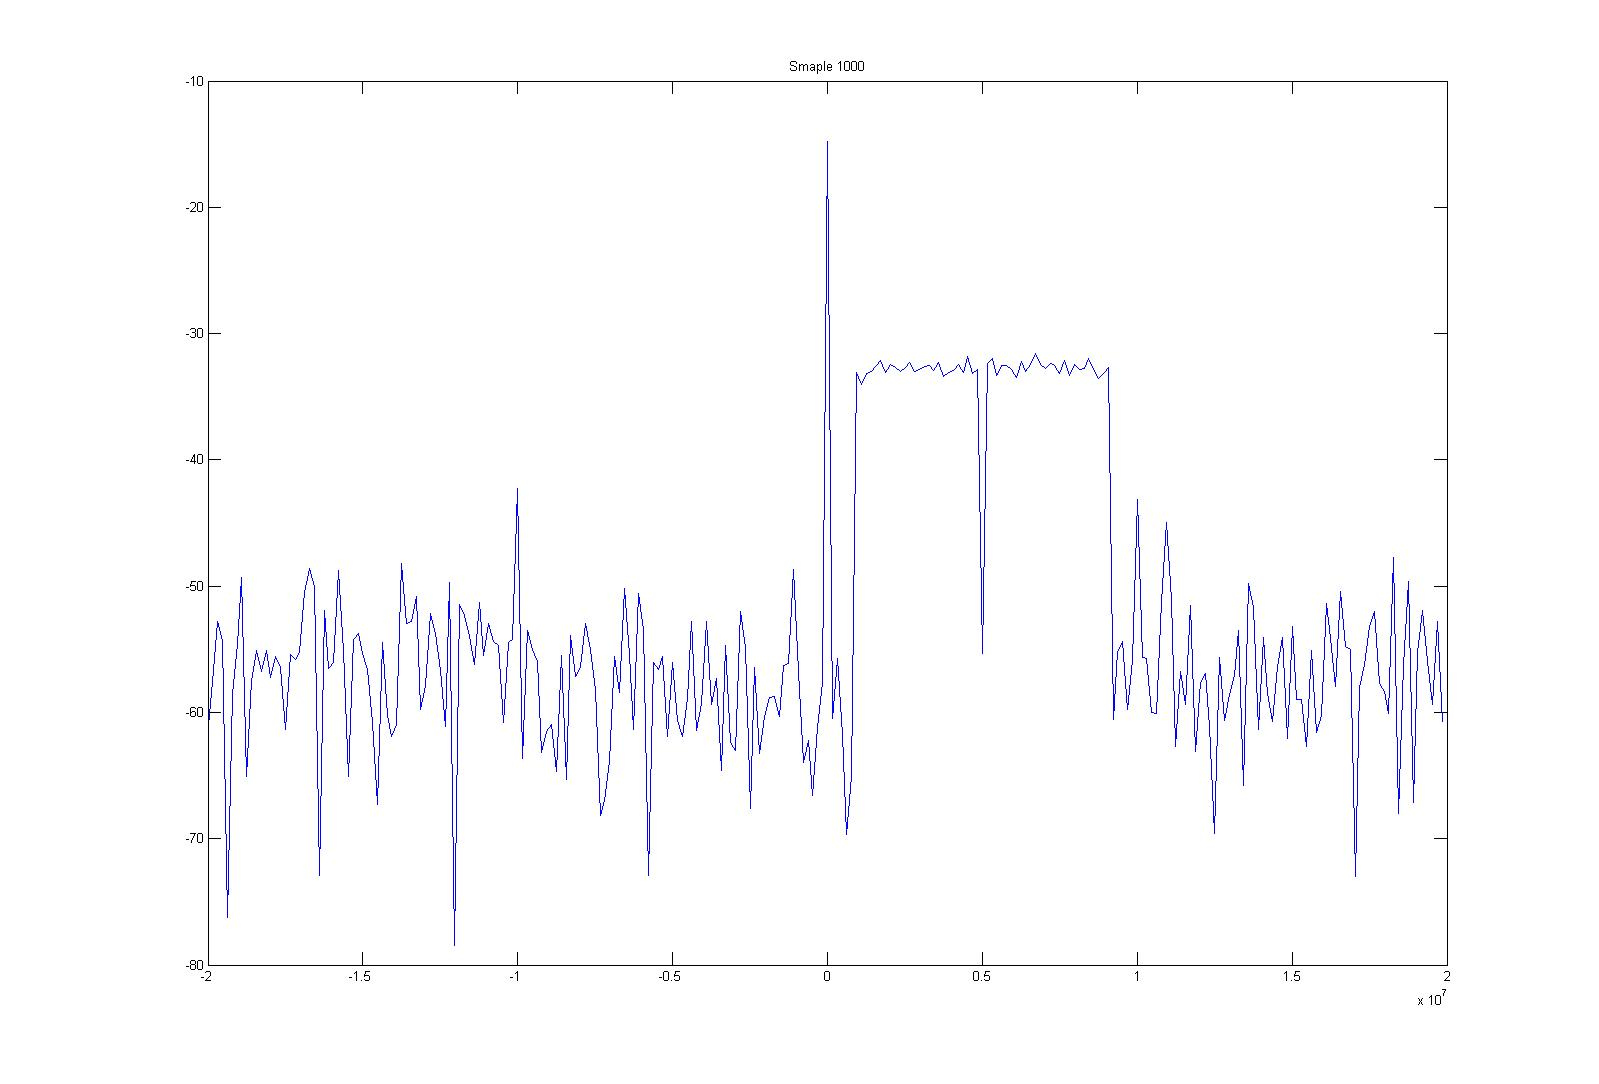
\includegraphics[width=\textwidth]{content/fig/RfIF.JPG}
\captionof{figure}{LTS Spectrum- passed RF chain (IF filter is enable)}
\label{RfIF}
\end{center}

\begin{center}
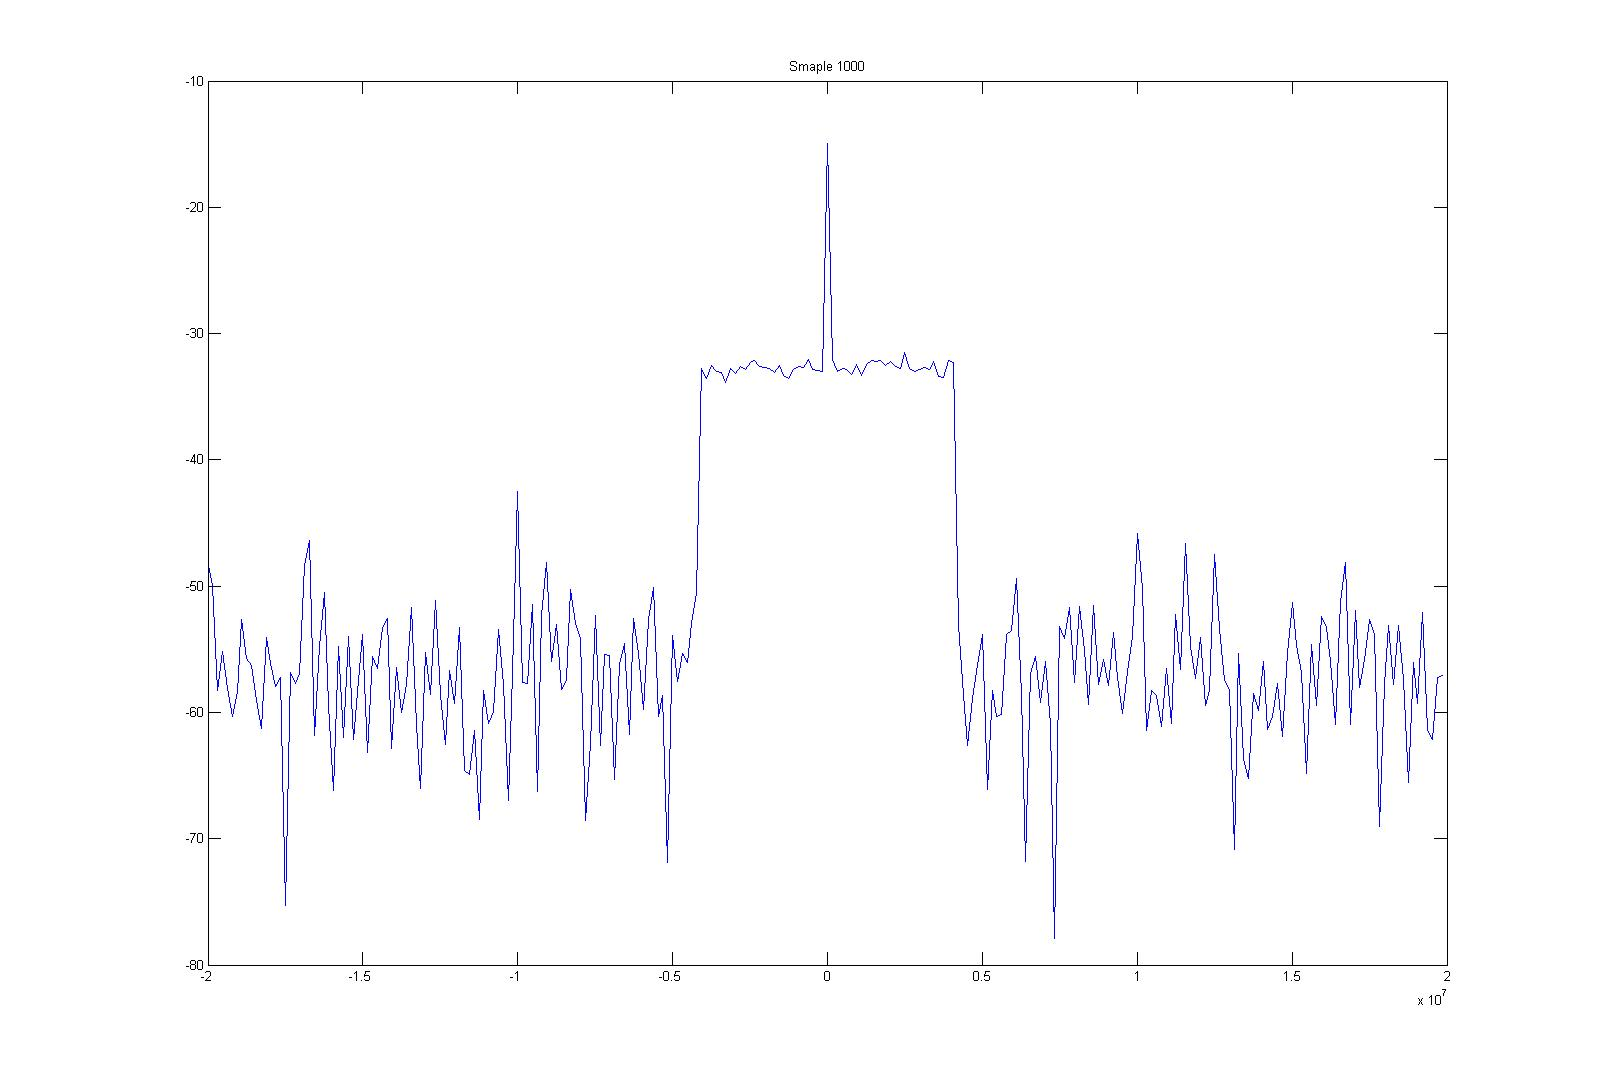
\includegraphics[width=\textwidth]{content/fig/Rfbase.JPG}
\captionof{figure}{LTS Spectrum- passed RF chain (IF filter is disable)}
\label{Rfbase}
\end{center}

\begin{center}
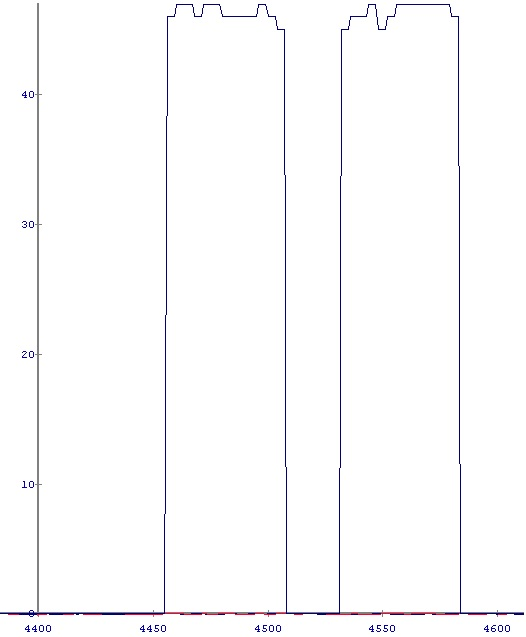
\includegraphics[width=\textwidth]{content/fig/h_mag_chipscope.JPG}
\captionof{figure}{Frequency Response of a semi-perfect channel}
\label{h_mag_chipscope}
\end{center}
%\zexternaldocument{part2}

\begin{abstract}
After explanation of the system architecture and hardware design, the test methodology and the analysis of the results from the hardware is defined. The results are captured thanks to ChipScope software which help for internal acquisitions in various points of the Programmable Logic of FPGA. There are other tests we did to have an estimation of the system in total. For instance, we send a random data stream from a PC and send it via Ethernet in different packet size to a board and compare it in another PC where we generate the same random set.\\
\end{abstract}

\section{Hardware Samples and Analysis}
\label{hw_samples}

A complete OFDM frame is illustrated in Figure \ref{ofdmframe_chipscope}. The position of preamble signal is completely distinguished in the figure which is comparable of the standard shown in previously except the \textit{Training}. This section is special for our design for conveying some further information about the node. The detail of each preamble word is zoom in the next figures as defined in Section \ref{section:ieee_standard}. Specifically, the STS section is shown in Figure \ref{sts_chipscope}.\\
\begin{center}
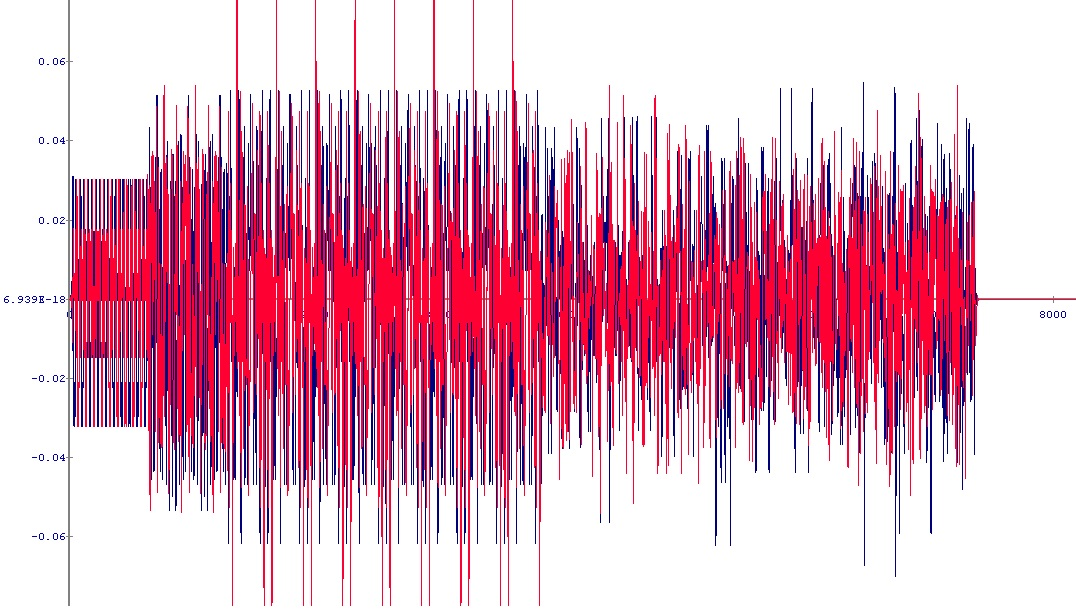
\includegraphics[width=\textwidth]{content/fig/ofdmframe_chipscope.JPG}
\captionof{figure}{OFDM Frame (I/Q) detected in Chipscope.}
\label{ofdmframe_chipscope}
\end{center}

\begin{center}
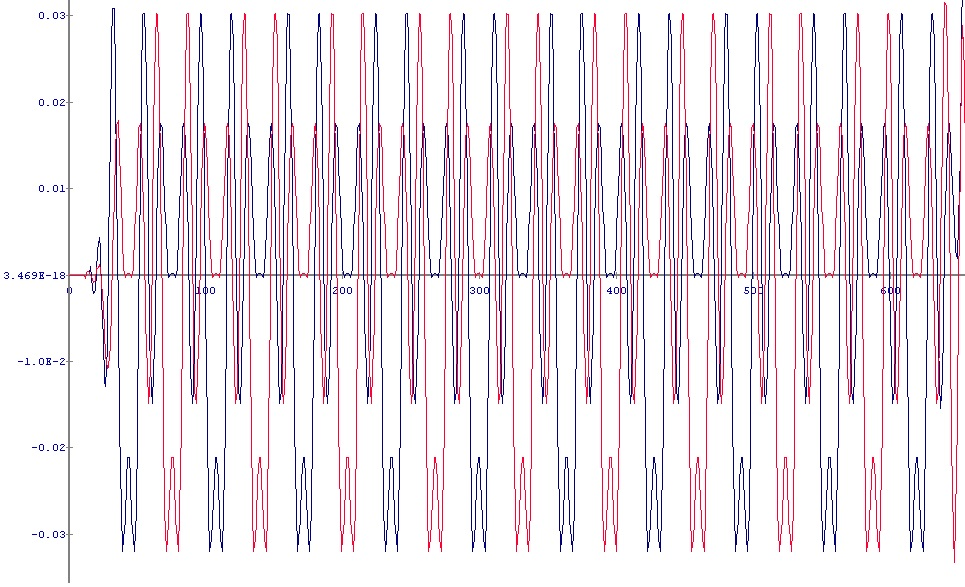
\includegraphics[width=12cm]{content/fig/sts_chipscope.JPG}
\captionof{figure}{STS (I/Q) detected in Chipscope.}
\label{sts_chipscope}
\end{center}

The auto-correlation is perform to catch the begining of the preamble with is STS. The output of the block is shown in Figure \ref{autocorr} to detect the signal arrival.\\

\begin{center}
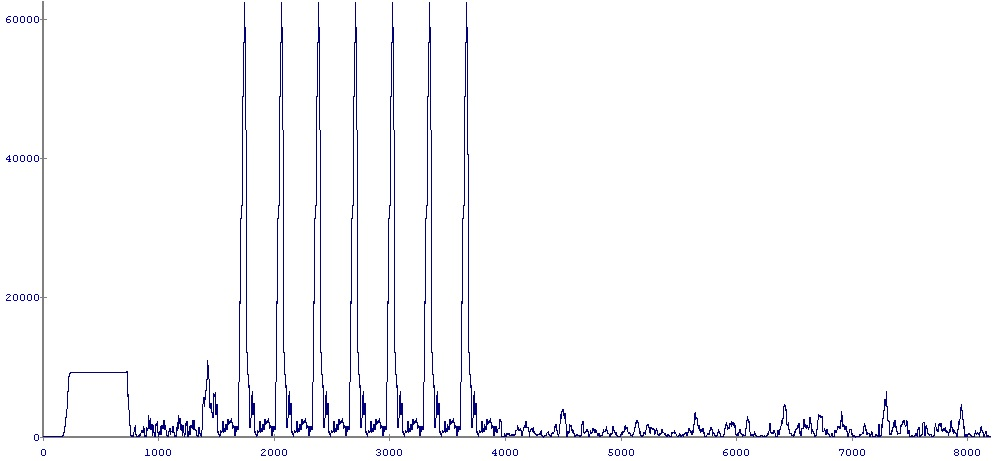
\includegraphics[width=\textwidth]{content/fig/autocorr.JPG}
\captionof{figure}{Auto-Correlation detected in Chipscope.}
\label{autocorr}
\end{center}

The cross-correlation on the LTS with a pre-defined expected LTS is shown in Figure \ref{crosscorr}. As already described we have 2.5 LTS symbol in each frame. So, two peak are detected in the system.\\

\begin{center}
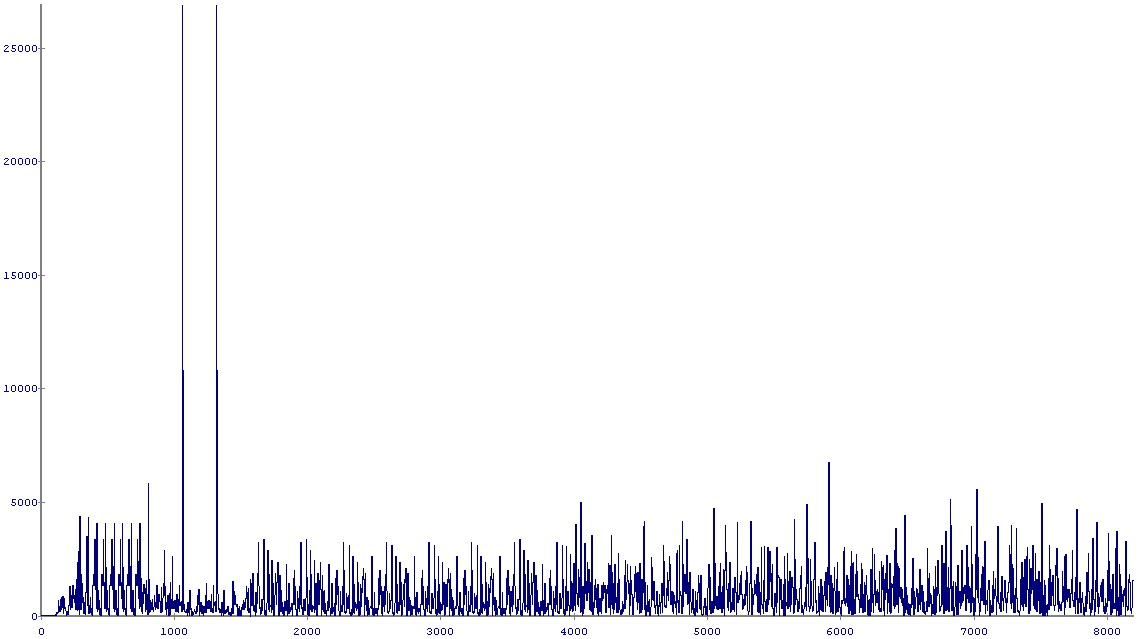
\includegraphics[width=\textwidth]{content/fig/crosscorr.JPG}
\captionof{figure}{Cross-Correlation detected in Chipscope.}
\label{crosscorr}
\end{center}

The LTS section is supposed to carry a flat shape in frequency that is used for the channel response estimation. In the Figure \ref{baseIFAdcDac} shows the frequency response of the LTS in the in the input of the receiver side. Beginning of the system test, we make a loop after the DAC of the transmitter to the ADC of the receiver and the is no RF conversion. Practically, this shape represents the frequency response of the ADC/ DAC and some non-linear elements like induction and trances. Because, there are some trances in the path who rejects the DC frequencies we needed to use an IF filter to modulate the signal around $5 MHz$.\\

\begin{center}
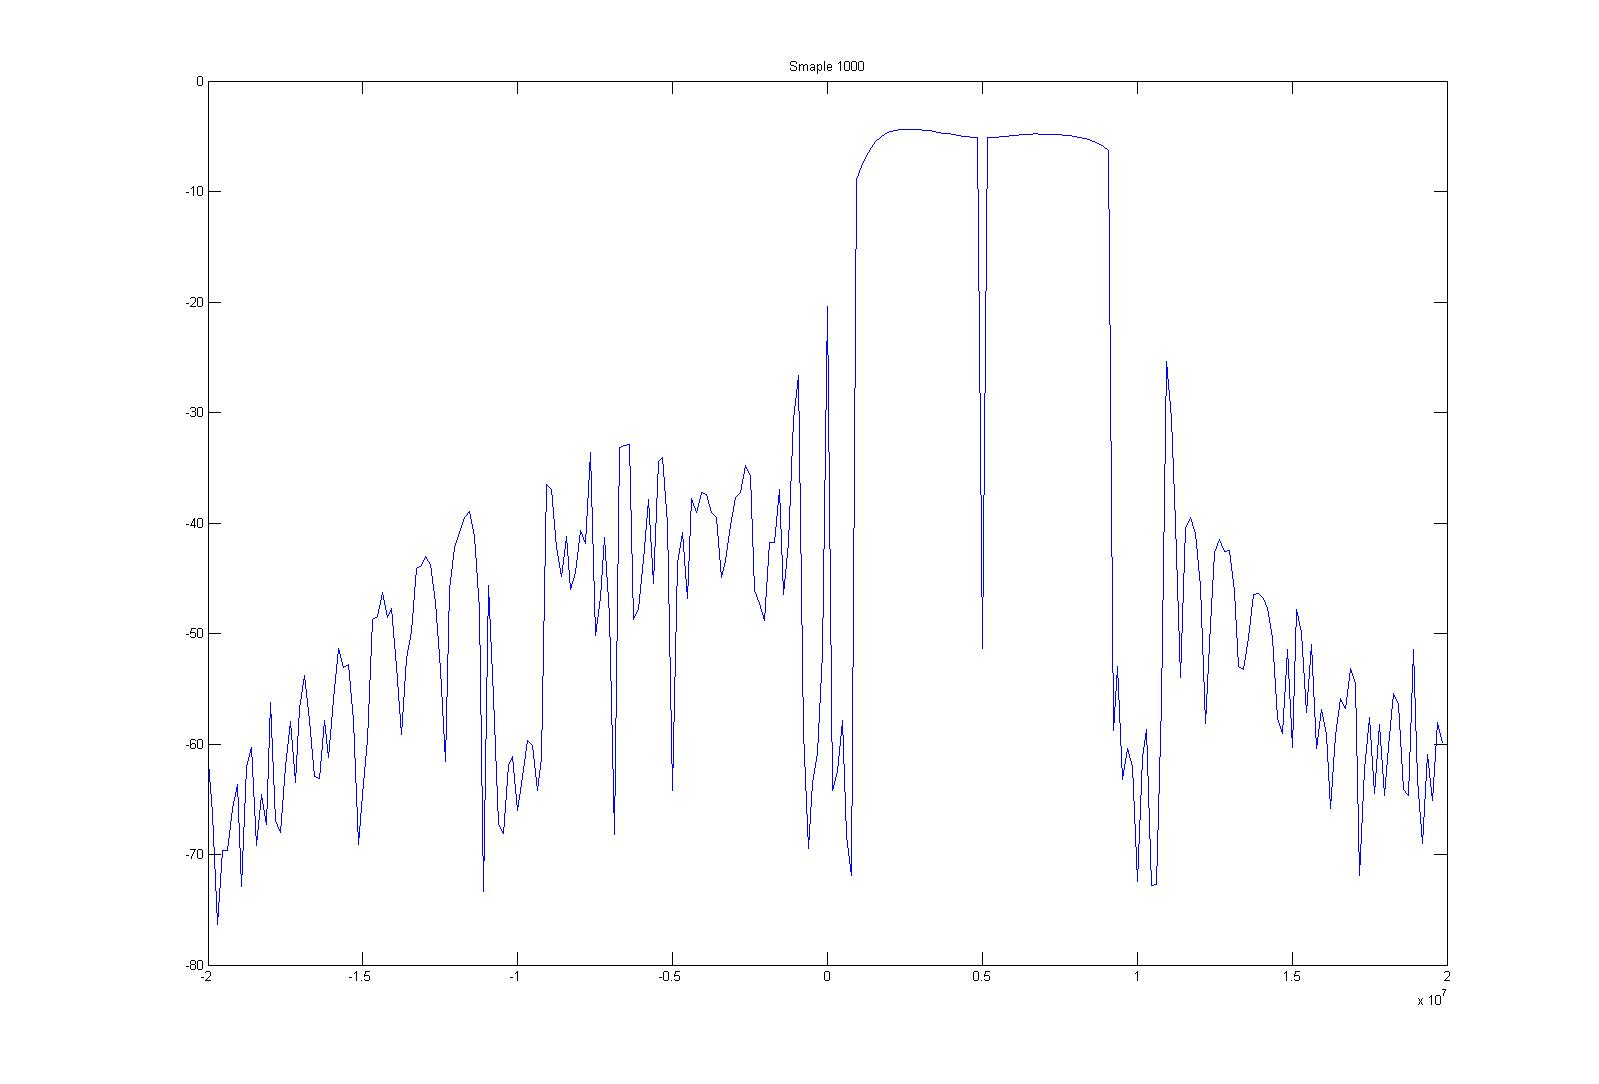
\includegraphics[width=10cm]{content/fig/baseIFAdcDac.JPG}
\captionof{figure}{LTS Spectrum in Baseband chain (IF filter on 5MHz is enable)}
\label{baseIFAdcDac}
\end{center}

Passing the signal through the RF side which modulate around $2.4 GHz$ and demodulate it again we have a shape as shown in Figure \ref{RfIF}. As you can see we still have the IF filter. The peak on 0 frequency is a result of the electronic elements which injects DC.\\

\begin{center}
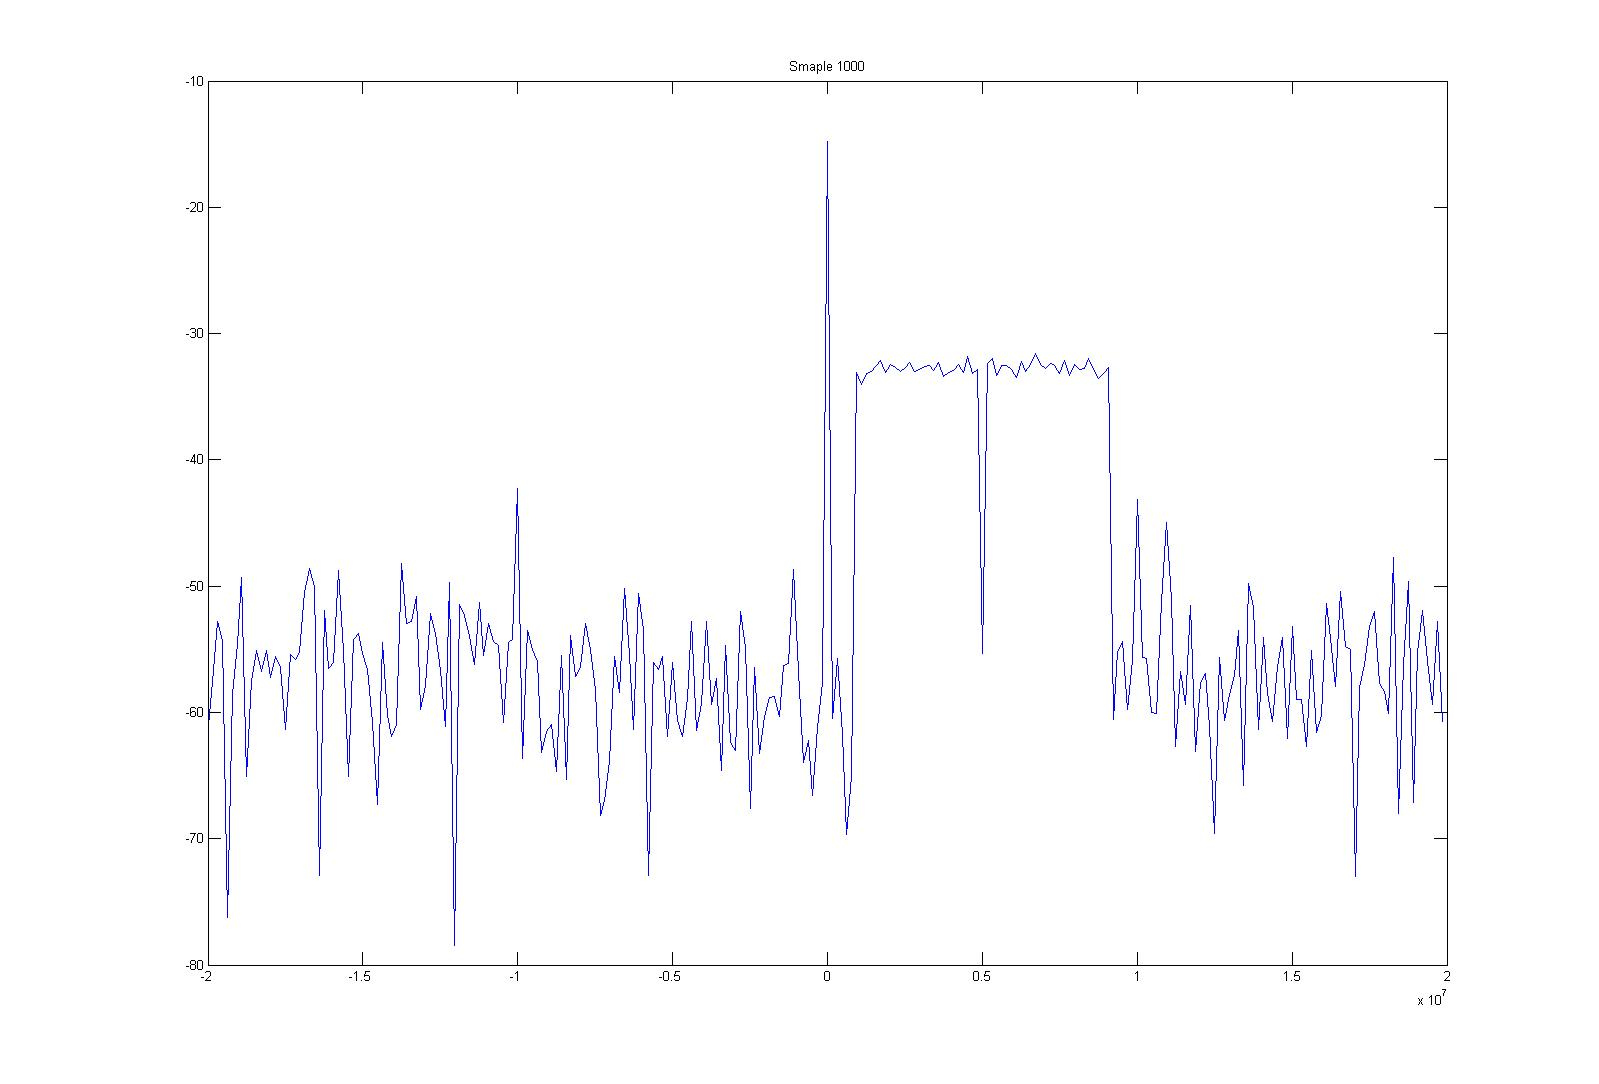
\includegraphics[width=10cm]{content/fig/RfIF.JPG}
\captionof{figure}{LTS Spectrum- passed RF chain (IF filter  on 5MHz is enable)}
\label{RfIF}
\end{center}

We have a shape of LTS frequency response like Figure \ref{Rfbase} if the IF filter is not activated. As you can see we have the DC peak which can be rejected easily.\\

\begin{center}
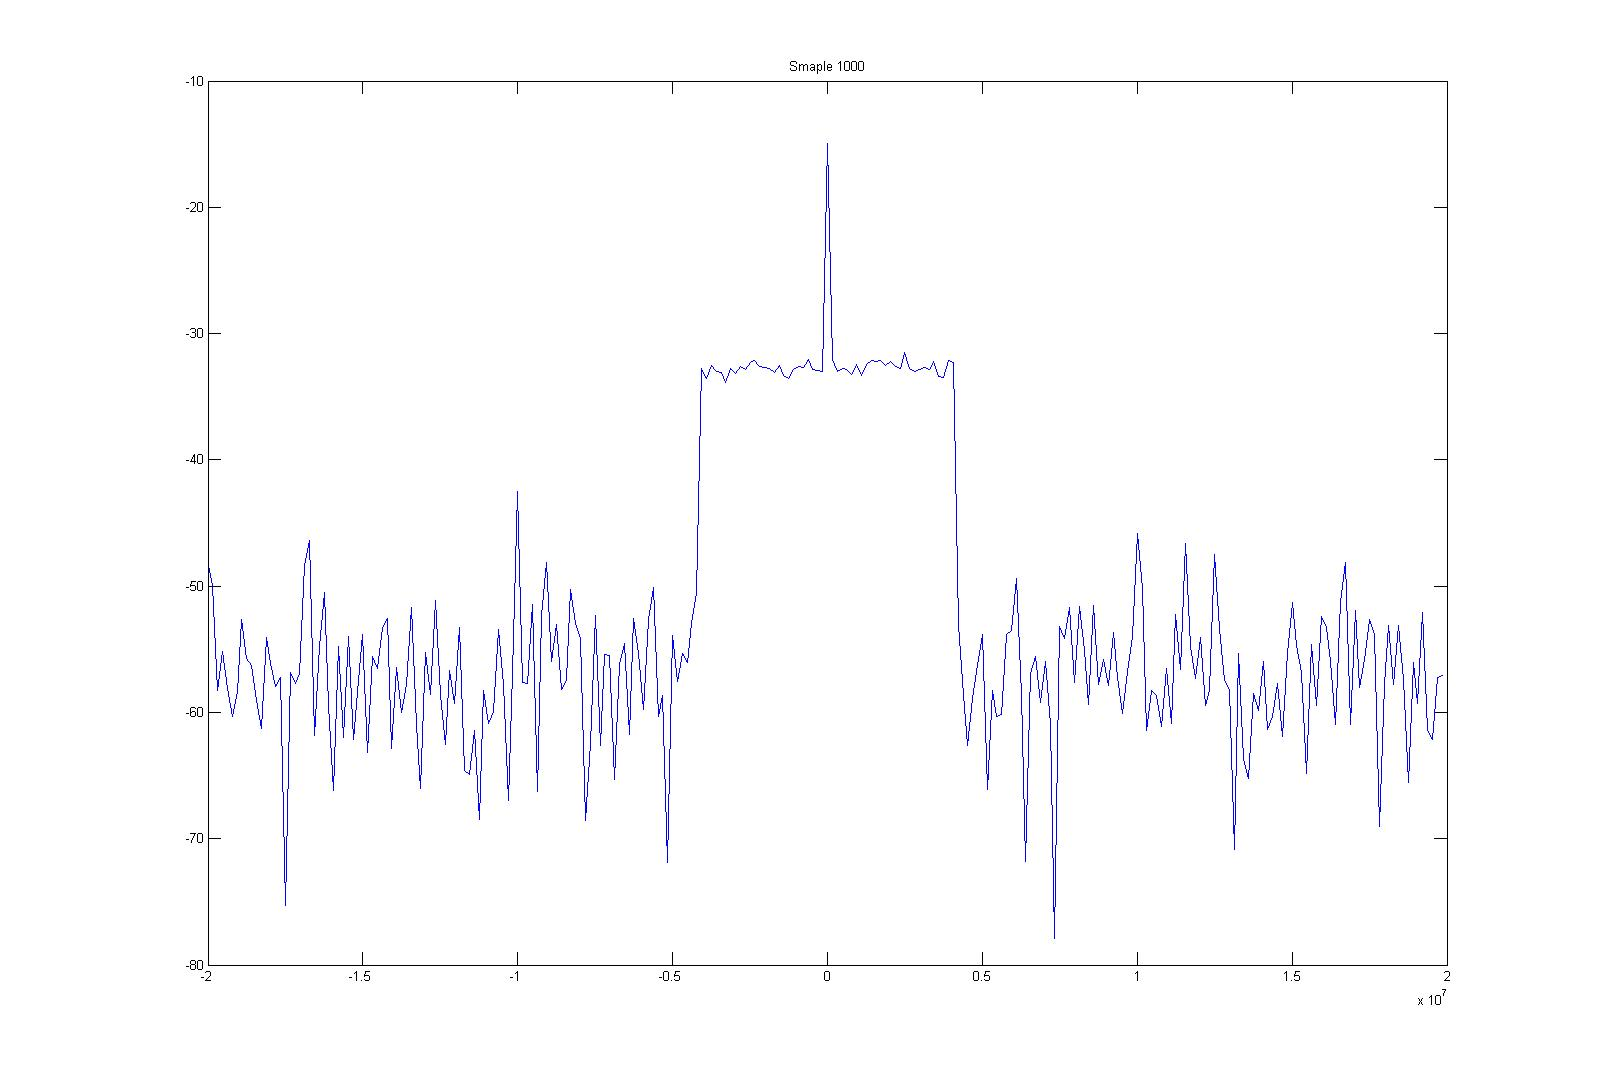
\includegraphics[width=10cm]{content/fig/Rfbase.JPG}
\captionof{figure}{LTS Spectrum- passed RF chain (IF filter is disable)}
\label{Rfbase}
\end{center}

Figure \ref{h_mag_chipscope_noChannel} is the frequency response of the channel after an internal loop between the transmitter and the receiver on one FPGA board. As it is a perfect channel without any distortion we just have a perfect flat estimation of the channel. This response is used to compensate all the signal tones.\\

\begin{center}
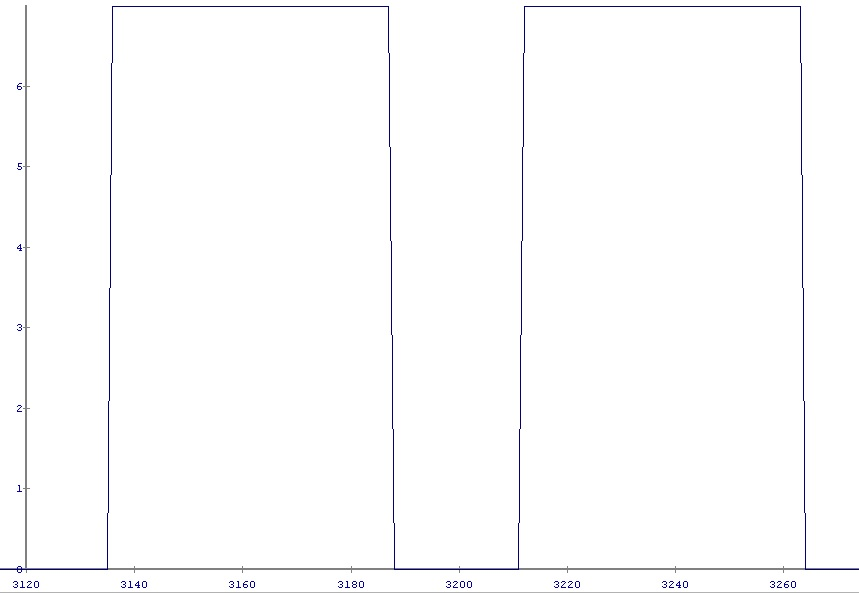
\includegraphics[width=10cm]{content/fig/h_mag_chipscope_noChannel.JPG}
\captionof{figure}{Frequency Response of a perfect channel detected in Chipscope}
\label{h_mag_chipscope_noChannel}
\end{center}

Figure \ref{h_mag_chipscope_rf_detect} in a real channel after all the conversions of the transmitter and the receiver. The RF chain is activated in the scenario. Interestingly, we have a perfect detection of the symbols even after such the distortion.\\

\begin{center}
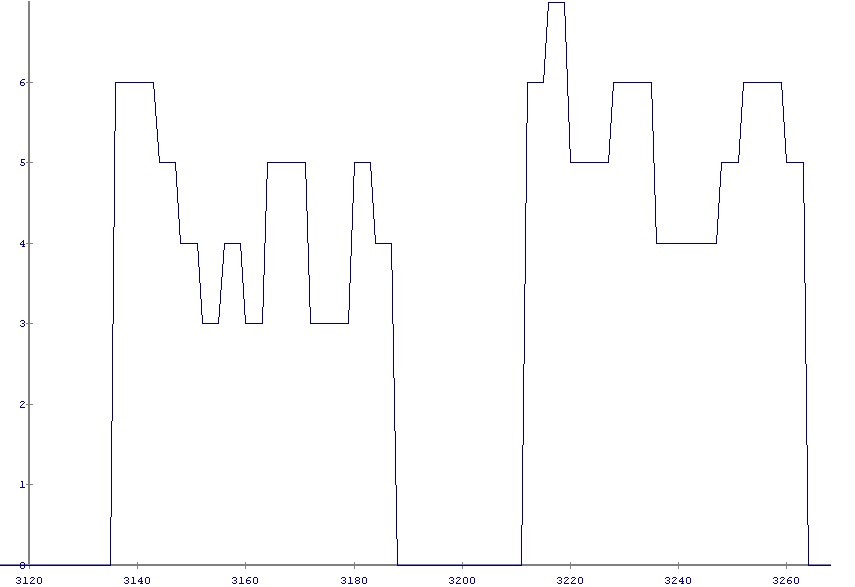
\includegraphics[width=10cm]{content/fig/h_mag_chipscope_rf_detect.JPG}
\captionof{figure}{Frequency Response of on air channel detected in Chipscope}
\label{h_mag_chipscope_rf_detect}
\end{center}

\begin{center}
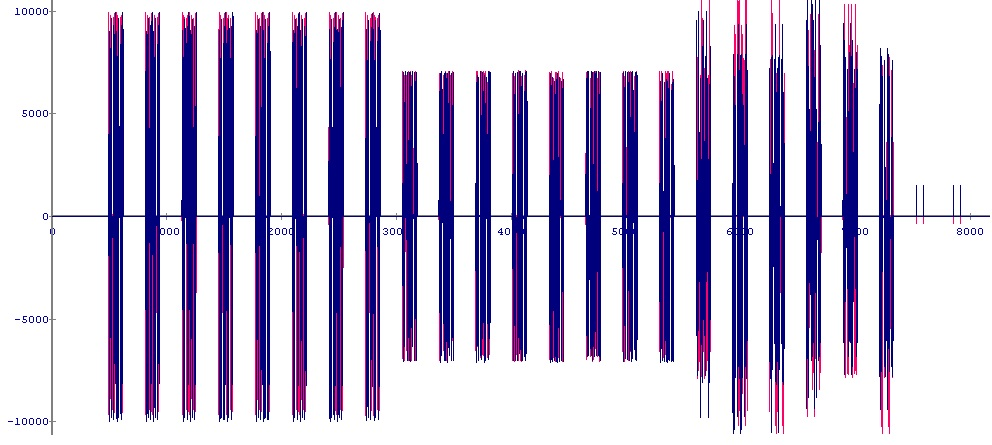
\includegraphics[width=\textwidth]{content/fig/OfdmSym_16qam_1_2_code_64byte.JPG}
\captionof{figure}{OFDM Symbols of a 16QAM 64-byte message Coded 1/2 rate}
\label{OfdmSym_16qam_1_2_code_64byte}
\end{center}

Figures \ref{OfdmSym_16qam_1_2_code_64byte} and \ref{OfdmSym_16qam_no_code_64byte} compares two OFDM frames after the FFT block on the receiver side. The coding algorithm is a convolutional code which borrowed from another model and seen as a black-box for our system. Just do not consider the first 8 symbols because they are the training block which are not defined in the standard and are the customization on our specific application. The next 8 frames in the coded and 4 in the non-coded are the base rate frames to report to the receiver about the modulation, size of message, sequence number and some other detection information. the rest are the message and the valuable information for the higher levels of the system.\\

\begin{center}
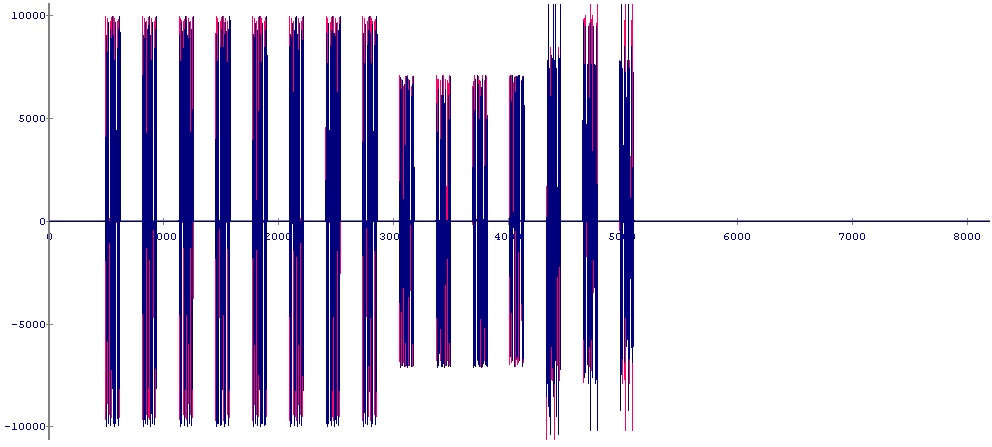
\includegraphics[width=\textwidth]{content/fig/OfdmSym_16qam_no_code_64byte.JPG}
\captionof{figure}{OFDM Symbols of a 16QAM 64-byte message no-Coded}
\label{OfdmSym_16qam_no_code_64byte}
\end{center}

\section{Bit-Error Rate Calculation}
Will be add later!!!


\section{FPGA Resource Consumption}
The device used in our implementation is  XC7Z045-22FFG900C and in Table \ref{table:DevUtil} you can find the device utilization:\\


\begin{center}
\captionof{table}{Device Utilization Summary (actual values)}
\label{table:DevUtil}
\vspace{0.5cm}
\begin{tabular}{c|c|c|c}
Slice Logic Utilization&Used&Available&Utilization\\ \hline
Number of Slice Registers&42,703&437,200&9\% \\
Number of Slice LUTs&59,787&218,600&27\% \\
Number used as Memory&5,384&70,400&7\% \\
Number of occupied Slices&21,749&54,650&39\% \\
Number of DSP48E1s&149&900&16\% \\
\end{tabular}
\end{center}

Keep in mind this table shows all the utilization of the ADC/DAC interface, BRAM, clock generator and OFDM PHY module. For OFDM PHY module we could reach Net Skew 0.51 ns and maximum  Delay $1.91 ns$. About the ARM processor, we used one of the ARM cores although we have a dual core architecture. It works with $666.6 MHz$ clock. It is almost 20\% of the processor.\\

\section{Conclusion}

This thesis has presented the theoretical analysis and simulation and  FPGA implementation details of a baseband OFDM system with channel estimation and timing synchronization. A radio board also is explained for the practical usage and proof of the feasibility. The OFDM system is prototyped based on IEEE 802.11a standard and transmits/receives signals on a 20 MHz bandwidth. The conceptual design is done in System Generator and ported on a FPGA. With QPSK modulation scheme, the system achieves a throughput of 24 Mbps.\\
Another critical part of the project is to reach an acceptable communication bit-rate in the processor side to the peripherals, more specifically Ethernet, for conveying data between two PC which is done perfectly.\\

\subsection{Future Work}
No doubt, System Generator is a very powerful tool for conceptual proof but is not still an industrial support. There are still difference in the Simulation in Matlab and what we have in the hardware. To overcome this issue we needed to make some changes to have a logical margin of the hardware difficulties. The resource consumption is not very optimized which expected to have better performance using VHDL programming. There are many low-level techniques to manage the power, speed and area which is not applicable in the system.\\
Some other problems like model-based system maintenance, extend for the future and the bug detection difficulties make us to hesitate to industrialized a System Generator model at the moment. However, the accuracy of the theory is done perfectly in the current mechanism.\\
There are some projects in the department to extend the model for MIMO system design which is a good starting point. Besides, they try to upgrade the FFT point to higher levels for better bandwidth usage. A customized radio board is in the future program activities.\\

% References
\cleardoublepage

\bibliographystyle{unsrt}
\bibliography{Thesis_Bibliography}	


%\newpage
%\appendix
%\appendixpage
%\chapter{Use cases}\label{appexdix:usecases}

%The appendix provides the representation 

\end{document}
